% ------------------------------------------
%  MASTER THESIS DISSERTATION
% ------------------------------------------
% Author:
%
% Advisors:
%
% ------------------------------------------
\documentclass[10pt,twoside,openright,a4paper]{report}
\usepackage{inputenc}
% Set document margins to 1in in all sides
\usepackage[margin=2.5cm]{geometry}
% Line spacing package
\usepackage{graphicx, helvet, hyperref, setspace}
\usepackage[portuguese,english]{babel}
\usepackage[acronym, toc]{glossaries}

% Built the glossary when the main file is built.
\makeglossaries
% Set main font to Arial
\renewcommand{\familydefault}{\sfdefault}
% Define keywords macro
\providecommand{\keywords}[1]{\textbf{Keywords:} #1}
% Define the NewPage macro
\newcommand*\NewPage{\newpage\null\thispagestyle{empty}\cleardoublepage}
% Abstract-en page numbering
\newcommand {\abstractEnglishPageNumber} {\thispagestyle{plain}\setcounter{page}{\abstractEnglishPage}}
% Abstract-pt page numbering
\newcommand {\abstractPortuguesePageNumber} {\thispagestyle{plain}\setcounter{page}{\abstractPortuguesePage}}

% Section numbering depth
\setcounter{secnumdepth}{2}
% Table of contents depth
\setcounter{tocdepth}{3}
% Set line spacing to 1.5cm
\onehalfspacing
% Page numbering
\pagestyle{plain}

% Glossary-File
% Glossary Definition

\newglossaryentry{MSc}{name={MSc}, description={Masters degree in the area of Science.}}

% Acronym-File
% Acronym Definition

% ADSL
\newacronym{ADSL}{ADSL}{Asymmetric Digital Subscriber Line}
% ALE
\newacronym{ALE}{ALE}{Application Level Events}
% AWS
\newacronym{AWS}{AWS}{Amazon Web Service}
% AWS
\newacronym{CPU}{CPU}{Computer Processing Unit}
% EC2
\newacronym{EC2}{EC2}{Elastic Cloud Computing}
% EPC
\newacronym{EPC}{EPC}{Electronic Product Code}
% EPCIS
\newacronym{EPCIS}{EPCIS}{Electronic Product Code Information System}
% ERP
\newacronym{ERP}{ERP}{Enterprise Resource Planning}
% FCServer
\newacronym{FCServer}{FCServer}{Filtering \& Collection Server}
% GB
\newacronym{GB}{GB}{Gigabyte}
% GHz
\newacronym{GHz}{GHz}{Gigahertz}
% H2M
\newacronym{H2M}{H2M}{human-to-machine}
% HTTP
\newacronym{HTTP}{HTTP}{Hypertext Transfer Protocol}
% IaaS
\newacronym{IaaS}{IaaS}{Infrastructure as a Service}
% LTE
\newacronym{LTE}{LTE}{Long-term Evolution}
% IoT
\newacronym{IoT}{IoT}{Internet of Things}
% LLRP
\newacronym{LLRP}{LLRP}{Low Level Reader Protocol}
% LXC
\newacronym{LXC}{LXC}{Linux Container}
% M2M
\newacronym{M2M}{M2M}{machine-to-machine}
% MB
\newacronym{MB}{MB}{Megabyte}
% NFC
\newacronym{NFC}{NFC}{Near Field Communication}
% NoSQL
\newacronym{NoSQL}{NoSQL}{Not Only SQL}
% OS
\newacronym{OS}{OS}{operating system}
% PaaS
\newacronym{PaaS}{PaaS}{Platform as a Service}
% PIQL
\newacronym{PIQL}{PIQL}{Performance Insightful Query Language}
% RAM
\newacronym{RAM}{RAM}{Random-access memory}
% RDBMS
\newacronym{RDBMS}{RDBMS}{Relational Database Management System}
% RFID
\newacronym{RFID}{RFID}{Radio-Frequency IDentification}
% SaaS
\newacronym{SaaS}{SaaS}{Software as a Service}
% ubicomp
\newacronym{ubicomp}{ubicomp}{Ubiquitous Computing}
% VM
\newacronym{VM}{VM}{Virtual Machine}
% WAN
\newacronym{WAN}{WAN}{Wide Area Network}


% ------------------------------------------
% MASTER THESIS DISSERTATION
% ------------------------------------------

\begin{document}
\pagenumbering{gobble}% Remove page numbers (and reset to 1)
\clearpage
\thispagestyle{empty}
%!TEX root = ./article.tex

% Article Title
\def \ArticleTitle{Cloud4Things}

% Author(s) Name(s)
\def \AuthorA{Marcus Vin\'icius Paulino Gomes}

% Author(s) Email(s)
\def \AuthorAemail{marcus.paulino.gomes@tecnico.ulisboa.pt}

% Institution(s) Name(s)
\def \InstitutionA{Instituto Superior T\'ecnico, Universidade de Lisboa}

% Article Title
\newcommand {\Title} {\ArticleTitle}

% Authors
\newcommand {\Authors} {\IEEEauthorblockN{\AuthorA}}

% Institution
\newcommand {\Institutions} {\IEEEauthorblockA{\InstitutionA}\\
                            Email: \AuthorAemail}

% Variable to control if the bibliography must be include
\def \hasBibliography{1}


%!TEX root = ./dissertation.tex

% ---------------------------------------------------------
%   MASTER THESIS DISSERTATION COVER
% ---------------------------------------------------------
\begin{titlepage}
% ---------------------------------------------------------
%  INSTITUTION LOGO
% ---------------------------------------------------------

\includegraphics[width=5cm]{images/ist_logo}~\\
%
\if\IsFinalVersion 1
  \vspace*{\finalLogoSpacing}
\else
  \vspace*{\draftLogoSpacing}
\fi

\begin{center}
% ---------------------------------------------------------
%  MASTER THESIS DISSERTATION TITLE
% ---------------------------------------------------------
{\LARGE \textbf{\Title}}\\[1.0cm]
% ---------------------------------------------------------
%  MASTER THESIS DISSERTATION SUBTITLE
% ---------------------------------------------------------
{\Large \Subtitle}\\[1.0cm]
% ---------------------------------------------------------
%  AUTHOR NAME (FULL)
% ---------------------------------------------------------
{\Large \textbf{\StudentName}}\\[1.0cm]
% ---------------------------------------------------------
%  DISSERTATION DEGREE
% -----------------------------------------------------------------
{\large Thesis to obtain the Master of Science Degree in}\\[1.0cm]
% -----------------------------------------------------------------
%  COURSE NAME
% -----------------------------------------------------------------
{\LARGE \textbf{\DegreeName}}\\[1.0cm]

% -----------------------------------------------------------------
%  ADVISORS NAME
% ---------------------------------------------------------
\begin{minipage}[t]{.4\textwidth}
  \center
  \begin{flushright}
    {\large Supervisors:~~}
  \end{flushright}
\end{minipage}%
\begin{minipage}[t]{.6\textwidth}
  \center
  \begin{flushleft}
    {\Supervisors}
  \end{flushleft}
\end{minipage}\\
%
\if\IsFinalVersion 1
  \vspace*{\finalAdvisorsSpacing}
\else
  \vspace*{\draftAdvisorsSpacing}
\fi
% ---------------------------------------------------------
%  JURI NAMES:
%  - PRESIDENT
%  - ADVISOR
%  - VOGALS
% ---------------------------------------------------------
\if\IsFinalVersion 1
%
\begin{minipage}[t]{1\textwidth}
  \center
  {\Large \textbf{Examination Committee}}\\[.25cm]
  {\large Chairperson: \Chairperson}\\
  {\large Supervisor: \MainSupervisor}\\
  {\large Member of the Committee: \CommitteeMembers}
\end{minipage}\\[1.0cm]
%
\fi

\if\IsFinalVersion 1
 \vspace*{\dateSpacing}
\fi

% ---------------------------------------------------------
%  DATE (MONTH AND YEAR)
% ---------------------------------------------------------
{\Large \textbf{\Month\:\Year}}\\
\end{center}
\end{titlepage}

\NewPage

\pagenumbering{roman}

% Acknowledgments Page
\setcounter{page}{\acknowledgmentsPage}
\if\includeAcknowledgments 1
%!TEX root = ../dissertation.tex

% Acknowledgments: This one is optional
\chapter*{Acknowledgments}
I would like to thank my advisors Prof. Miguel Pardal and Prof. Jos\'e Alves
Marques that helped me in the development of this Master Thesis.
In special, I want to thank Prof. Miguel Pardal for the given support
throughout this year and specially in the writing of this document. I also
would like to thank the members of committee that evaluated this work and
provided feedback.\\

Finally, I would like to thank my mother for supporting me during these last 5
years and my friends and colleagues that supported me throughout my academic
path.

\NewPage
\fi

% Abstract - English
%!TEX root = ../dissertation.tex

\begin{otherlanguage}{english}
\begin{abstract}
Your abstract goes here.

% Keywords
\begin{flushleft}

\keywords{my keywords}

\end{flushleft}

\end{abstract}
\end{otherlanguage}

\NewPage

% Abstract - Portuguese
%!TEX root = ../dissertation.tex

\begin{otherlanguage}{portuguese}
\begin{abstract}
% Enable page numbering
\abstractPortuguesePageNumber
O teu resumo aqui...

% Keywords
\begin{flushleft}

\keywords{as tuas palavras chave}

\end{flushleft}

\end{abstract}
\end{otherlanguage}

\NewPage

% Table of contents
\tableofcontents

% List of Table
\addcontentsline{toc}{chapter}{\listtablename}
\listoftables
\NewPage

% List of figures
\addcontentsline{toc}{chapter}{\listfigurename}
\listoffigures
\NewPage

% List of acronyms
\printglossary[type=\acronymtype]
\NewPage

\pagenumbering{arabic}% Arabic page numbers (and reset to 1)
%!TEX root = ../dissertation.tex

% Entry point for chapters
% In this file you define the order
% in which the chapters are included

% Chapters
%!TEX root = ../dissertation.tex

\chapter{Introduction}
\label{chapter:introduction}
In recent years, computing is becoming more ubiquitous in the physical world. This notion where
computational elements are embedded seamlessly in ordinary objects that are connected through a
continuous network was introduced many years ago \cite{weiser1991computer}. The progress
towards ubiquitous computing has been slower than expected, technology advances such as the mobile
Internet contributes to achieve this vision in which computational devices are able to communicate
between themselves from any part of the world \cite{gubbi2013internet}. In this vision, an ubiquitous
system is composed of physical items that are continuously connected to the virtual world and can act as
remotely and physical access points to Internet Services \cite{mattern2010internet}.\\

However, there are some challenges that must be addressed in order to make these \gls{ubicomp} systems
truly ubiquitous \cite{caceres2012ubicomp}. An important concern regards about ubiquitous data: \textit{Where it is located?},
\textit{Who can access it?} and \textit{How much time this data should persist?}. Also, ubiquitous systems
are constantly interacting with the surrounding environment, thus these systems need to understand
the context in that they are inserted and also to adapt to the changes that occur in this environment.
Another import concern regards about the infrastructure burden of the ubiquitous systems. These
systems requires low-latency interaction with users and environments, which implies that at least part
of an \gls{ubicomp} application needs to be tightly bounded to the local infrastructure of the interacting
environment. This requirement for local infrastructure is a barrier in the adoption of ubiquitous
systems in a large-scale perspective.\\

This ubiquitous world is close to becoming reality thanks to the Utility Computing in the cloud
and the \gls{IoT}. In one hand, the utility computing provides the illusion of infinite computing
resources available on demand to the public users \cite{armbrust2010view}, which helps to reduce the
infrastructure burden of the ubiquitous systems. In the other hand the \gls{IoT} aims to solve a key
problem in wider adoption of ubiquitous systems, the tight coupling with a particular embedded
infrastructure. With the \gls{IoT} a variety of \textit{objects} or \textit{things} - such as \gls{RFID},
tags, sensors, actuators, etc. - will be able to interact with each other and cooperate with the
surrounding \textit{things} to reach common goals \cite{atzori2010internet}.\\

% Motivation
\section{Motivation}
\label{section:motivation}
This recent progress in the utility computing and the Internet of Things has been contributing to grow the
\gls{ubicomp} infrastructure. However, it is possible to identify new challenges \cite{caceres2012ubicomp}
for the construction of ubiquitous systems that arises from the integration of the Internet of Things
in the utility computing:

% Challenges
\begin{itemize}
  % Low-latency Interaction
  \item \textbf{Low-latency Interaction} is a key requirement of \gls{IoT} systems. In cloud-based
  solutions, part of the system's infrastructure is moved to the cloud - for instance the middleware layer,
  which is responsible for processing the information and take automatic decisions based on the results
  - is not possible to guarantee that the low-latency requirements of \gls{IoT} systems will be
  met for a cloud-based solution.
  % Scalable Data Storage
  \item \textbf{Data} is continuously generated by the \textit{things} that composes the \gls{IoT}
  system. That data must be stored, processed and presented in an seamless and efficient way. Several
  middleware solutions for \gls{IoT} \cite{floerkemeier2007rfid}\cite{eisenhauer2010hydra}\cite{de2008socrades}
  rely on consistent transactions supported by \glspl{RDBMS}, which unfortunately is not scalable
  \cite{hofmann2010cloud}. Since there is no industrial-grade solution for applications that rely on
  consistent transactions to write in multiple nodes at the same time, running high-volume, mission-critical
  transactional systems in the cloud is not a viable option.
  % Infrastructure Provisioning
  \item \textbf{Infrastructure Provisioning} usually was performed in a physical, isolated and vertical
  manner, in which hardware, networks, middleware and application logics are tightly coupled. Recently,
  \gls{IoT} has been adopted more and more in business and tends to weave into our daily life through the smart cities
  \cite{caragliu2011smart}\cite{schaffers2011smart}, this provisioning model presents some limitations
  that makes the delivery of new services an inefficient process, since that each time the same process
  has to be repeated to develop and deploy a new vertical solution.
  % Management
  \item \textbf{Management} of IoT systems is an issue that must be carefully addressed. In one hand
  is already proved that end-users are unable to manage their own personal computers systems well
  \cite{doll1988measurement}. Since there is no reason to believe that they will had a better
  performance at managing a much more complex system - such as an \gls{IoT} system - is reasonable to
  assume service providers will perform the management of the services . In the other hand, if we
  consider applications that are deployed in large-scale - such as smart cities - these managed
  services introduces new questions that must be answered. For instance, who will pay for this
  services and who will control this services?
  % Investment
  \item \textbf{Investment} in infrastructure is a relevant part of building an \gls{IoT} system,
  is this system deployed in a an small business or in a entire city. Is reasonable to assume that
  these investments need to be repaid. For instance, for businesses the return of investment is
  achieved with the improvement of its business processes, which can help to reduce the manufacturing
  cost of goods, to increase the efficiency of the supply chain, etc. However, for a large-scale
  system that is available for the general public a new model that is beneficial for both users and
  providers need to be established.
\end{itemize}

We believe that finding a solution to these problems is essential to the adoption of \gls{IoT} systems
in a large-scale perspective. However, some of these problems has a socio-economical nature - such as
management and investment of \gls{IoT} systems - and will take time to resolve this issues.

% Related Work
\section{Related Work}
\label{section:related_work}
Recently a lot of research and effort has been dedicated to solve these existing problems. In this
section we will present a summary of the most relevant related work that address to solve the
problems of converging the Internet of Things and the utility computing:

% Infrastructure Provisioning
\subsection{Infrastructure Provisioning}
\label{sub:provisioning}
The research area for infrastructure provisioning of IoT solutions is the one that presents the most
notable progress until now.

% Soldatos
\subparagraph{Soldatos} et al. \cite{soldatos2012convergence} presented the idea of converging the IoT and the utility computing in the
cloud. The proposed architecture is the core concept of the OpenIoT Project\footnote{http://openiot.eu},
and is based on CoAP \cite{shelby2014constrained} and linked data. The cloud is used at infrastructure
level, which allows to measure the utility of the services provided by inter-connected objects.
% Distefano
\subparagraph{Distefano} et al. \cite{distefano2012enabling} proposes an conceptual architecture by mapping various
elements in both clouds and IoT to the three layers of cloud architecture (\gls{PaaS}, \gls{SaaS} and \gls{IaaS}).
In this proposal IoT resources are provided voluntarily by their owners, while management functions
- such as node management and policy enforcement - are viewed as peer functions of cloud infrastructure
management. IoT resources and cloud infrastructure are mashed up for applications, which are delivered
through \gls{SaaS}.
% CloudThings
\subparagraph{CloudThings} \cite{zhou2013cloudthings} is an architecture that uses a common
approach to integrate Internet of Things and Cloud Computing. The proposed architecture is an online
platform which accommodates \gls{IaaS}, \gls{PaaS}, \gls{SaaS} and allows system integrators and
solution providers to leverage the complete application infrastructure for developing, operating
and composing applications and services.
% IoT PaaS
\subparagraph{Li} et. al \cite{li2013efficient} proposed IoT PaaS, a cloud platform that supports
scalable IoT service delivery. Solution providers are able to deliver new solutions by leveraging
computing resources and platform services - domain mediation, application context management, etc.
- on the cloud. The proposed architecture aims to enable virtual vertical service delivery, for that
it has a multi-tenant nature which is designed to help at the isolation of the environments of
different solutions.\\
% Scalable Data Storage
\subsection{Scalable Data Storage}
\label{sub:data_storage}
Since that no general solution for scalable data storage and retrieval in the cloud was developed,
cloud providers started to implement its own solutions.

\subparagraph{Google Big Table, Facebook Cassandra and  Amazon Dynamo} \cite{chang2008bigtable} \cite{lakshman2010cassandra}
\cite{decandia2007dynamo} are key-value stores - \gls{NoSQL} databases - that has the ability to horizontally scale - i.e,
distribute both data and load of simple operations through many servers - but it has a weaker concurrency model
than the ACID transactions of most \glspl{RDBMS} systems \cite{cattell2011scalable}.

\subparagraph{\gls{PIQL}} \cite{armbrust2010piql} is a SQL-like API
built to run on top of existing performance predictable key-value stores, that provides many of the benefits
using a traditional \gls{RDBMS}, such as the ability to express the queries in a declarative way, automatic
data parallelism, physical data independence and automatic index selection and maintenance, all while
maintaining the soft real-time guarantees on application performance that come from the underlying
key-value store.\\

Recently, some progress has been reached as regards scalable storage for \gls{RDBMS} systems. Although
most of the work still are in development, it is possible to highlight some solutions that are in a more
mature state.

\subparagraph{MySQL Cluster} \cite{ronstrom2004mysql} is a in-memory clustered distributed \gls{RDBMS}. Compared with
the MySQL implementation it works by replacing the InnoDB engine with the NDB - a proprietary
distributed layer from MySQL. MySQL Cluster is built on top of a shared-nothing architecture and includes
features such as failover, node recovery, synchronous data replication and no single point of failure.
MySQL Cluster seem to be the solution that scales to more nodes than other \gls{RDBMS} - 48 is the limit -
it was reported that after scaling up to a few dozen nodes it starts to running into bottlenecks \cite{bunch2010evaluation}.

\subparagraph{VoltDB} \cite{stonebraker2013voltdb} is a \gls{RDBMS} designed for performance and scalability. VoltDB
assumes a multi-node cluster architecture where the tables are partitioned over multiple servers. Tables
can be replicated over servers - e.g. for fast access to data - shards are always replicated -
to recovery the data in case of a node crash - and database snapshots are supported. Currently some
features still are missing - online schema changes are limited and asynchronous WAN replication and
recovery are not yet implemented - but in its current implementation VoltDB already presents some
features that improves the performance of SQL execution, as result the number of nodes that are needed
to support a given application load can be reduced in a significant way.

% Low-latency Interaction
\subsection{Low-latency Interaction}
\label{sub:low_latency_interaction}
Talk about this requirement through the different applications domain, i.e, each domain have its own
requirements for low-latency interaction.
% Objectives
\section{Objectives}
\label{section:objectives}
In this section I want to specify the application domain - RFID smart places - and describe the
objectives of our work.
% Document Structure
\section{Thesis Outline}
\label{section:outline}
The remainder of this document is organized as follows:
% Document structure item list
\begin{itemize}
  \item \textbf{Chapter \ref{chapter:background} Background}
  \item \textbf{Chapter \ref{chapter:implementation} Implementation}
  \item \textbf{Chapter \ref{chapter:evaluation} Evaluation}
  \item \textbf{Chapter \ref{chapter:conclusion} Conclusion}
\end{itemize}

%!TEX root = ../dissertation.tex

\chapter{Background}
\label{chapter:background}
This chapter presents the background necessary to comprehend the developed work. The first section
presents the related work relevant regarding to solve the challenges of converging the Internet of
Things and the Utility Computing. The following sections presents a description of the concepts
that composes the basis of our work.

% Related Work
\section{Related Work}
\label{section:related_work}
Recently a lot of research and effort has been dedicated to solve these existing problems. In this
section we will present a summary of the most relevant work that relates to the Internet of Things and the utility computing:

% Service Delivery
\subsection{Service Delivery}
\label{sub:service_delivery}
As referred in Section~\ref{section:motivation}, current \gls{IoT} solutions are delivered in a physical
and isolated manner, which makes its service delivery model an inefficient and unscalable process.
In order to turn the service delivery of \gls{IoT} solutions more efficient and scalable, cloud service
delivery models are being developed based on the existing layers of the cloud architecture \cite{zhang2010cloud}:
\textit{a) \gls{IaaS}} refers to the provisioning of infrastructure resources on-demand - e.g. \glspl{VM},
storage and network. \textit{b) \gls{PaaS}} refers to providing platform layer resources such as operating
system support and software development frameworks. \textit{c) \gls{SaaS}} refers to providing on demand
application over the Internet.

% Soldatos
\subparagraph{Soldatos} et al. \cite{soldatos2012convergence} presented the idea of converging the IoT
and the utility computing in the cloud. The proposed architecture is the core concept of the OpenIoT
Project\footnote{http://openiot.eu}, and is based on CoAP \cite{shelby2014constrained} and linked data.
The cloud is used at infrastructure level, which allows to measure the utility of the services provided
by inter-connected objects.
% Distefano
\subparagraph{Distefano} et al. \cite{distefano2012enabling} proposed a conceptual architecture by
mapping various elements in both cloud and IoT to the three layers of cloud architecture (\gls{PaaS},
\gls{SaaS} and \gls{IaaS}). In this proposal IoT resources are provided voluntarily by their owners,
while management functions - such as node management and policy enforcement - are viewed as peer
functions of cloud infrastructure management. A \gls{PaaS} module is responsible to mashup IoT resources
and cloud infrastructure (\gls{IaaS}) for applications, which are delivered through \gls{SaaS}.
% CloudThings
\subparagraph{CloudThings} \cite{zhou2013cloudthings} is an architecture that uses a common
approach to integrate Internet of Things and Cloud Computing. The proposed architecture is an online
platform which accommodates \gls{IaaS}, \gls{PaaS}, \gls{SaaS} and allows system integrators and
solution providers to leverage the complete application infrastructure for developing, operating
and composing applications and services.
% IoT PaaS
\subparagraph{Li} et. al \cite{li2013efficient} proposed IoT PaaS, a cloud platform that supports
scalable IoT service delivery. Solution providers are able to deliver new solutions by leveraging
computing resources and platform services - domain mediation, application context management, etc.
- on the cloud. The proposed architecture aims to enable virtual vertical service delivery, for that
it has a multi-tenant nature which is designed to help at the isolation of the environments of
different solutions.\\

Although great progress was achieved regarding the improvement of service delivery for \gls{IoT}
solutions, most of the work still are in a conceptual stage. What is certain is that cloud service
delivery models will be the foundation for the service delivery models for \gls{IoT}.

% Data Storage Performance
\subsection{Data Storage Performace}
\label{sub:data_storage}
Since that data storage and retrieval in the cloud had specific requirements, cloud providers started
to implement their own solutions.

\subparagraph{Google Big Table, Facebook Cassandra and  Amazon Dynamo} \cite{chang2008bigtable} \cite{lakshman2010cassandra}
\cite{decandia2007dynamo} are key-value stores - \gls{NoSQL} databases - that has the ability to horizontally scale - i.e,
distribute both data and load of simple operations through many servers - but it has a weaker concurrency model
than the ACID transactions of most \glspl{RDBMS} systems \cite{cattell2011scalable}.

\subparagraph{\gls{PIQL}} \cite{armbrust2010piql} is a SQL-like API built to run on top of existing
performance predictable key-value stores, that provides many of the benefits of using a traditional
\gls{RDBMS}, such as the ability to express the queries in a declarative way, automatic data
parallelism, physical data independence and automatic index selection and maintenance, all while
maintaining the low latency guarantees on application performance that come from the underlying
key-value store.\\

Recently, some progress has been reached as regards scalable storage for \gls{RDBMS} systems. Although most
of the works still are in development, it is possible to highlight some solutions that are in a more
mature state.

\subparagraph{MySQL Cluster} \cite{ronstrom2004mysql} is an in-memory clustered distributed \gls{RDBMS}.
Compared with the MySQL implementation it works by replacing the InnoDB engine with the NDB - a proprietary
distributed layer from MySQL. MySQL Cluster is built on top of a shared-nothing architecture and includes
features such as failover, node recovery, synchronous data replication and no single point of failure.
MySQL Cluster seem to be the solution that scales to more nodes than other \gls{RDBMS} - 48 is the limit.
However, it was reported that after scaling up to a few dozen nodes it starts to running into
bottlenecks \cite{bunch2010evaluation}.

\subparagraph{VoltDB} \cite{stonebraker2013voltdb} is a \gls{RDBMS} designed for performance and scalability.
VoltDB assumes a multi-node cluster architecture where the tables are partitioned over multiple servers.
Tables can be replicated over servers - e.g. for fast access to data - shards are always replicated -
to recovery the data in case of a node crash - and database snapshots are supported. Currently some
features still are missing - online schema changes are limited and asynchronous \gls{WAN} replication and
recovery are not yet implemented - but in its current implementation VoltDB already presents some
features that improves the performance of SQL execution, as result the number of nodes that are needed
to support a given application load can be reduced in a significant way.

% Low-latency Interaction
\subsection{Low-latency Interaction}
\label{sub:low_latency_interaction}
Finding a general solution for the low-latency requirement of \gls{IoT} systems is not a easy task.
Since there are several application domains, it is natural that each application domain requires
that different values for network latency and data transmission latency are guaranteed.
% Talk about fog computing

 % Concepts
\section{Concepts}
\label{sec:Concepts}
This section presents the basics concepts that are relevant in the developed work. First, we start by
introducing the Fog Computing platform. Then, we present a description of the middleware platforms that
supports the \gls{RFID} technology. To end, we conclude with a brief description of the \glspl{LXC} technology
and the configuration management tools.

% Fog Computing
\subsection{Fog Computing}
\label{sub:fog_computing}
The Fog Computing \cite{bonomi2012fog} is a platform that aims to bring the cloud close to the ``Edge
of the Network''. By extending the cloud close to the ground, the Fog will be able to meet the requirements
of several applications that the traditional cloud is not able to accomplish. The most notable case
is the Internet of Things, that requires mobility support, geo-distribution in addition to location
awareness and low latency. The Fog achieves that by virtualizing the computing, storage and network
services between end devices and the traditional data centers in the cloud, that are not exclusively
located at the edge of the network.\\

% Fog Computing Infrastructure
\begin{figure}[ht!]
  \centering
  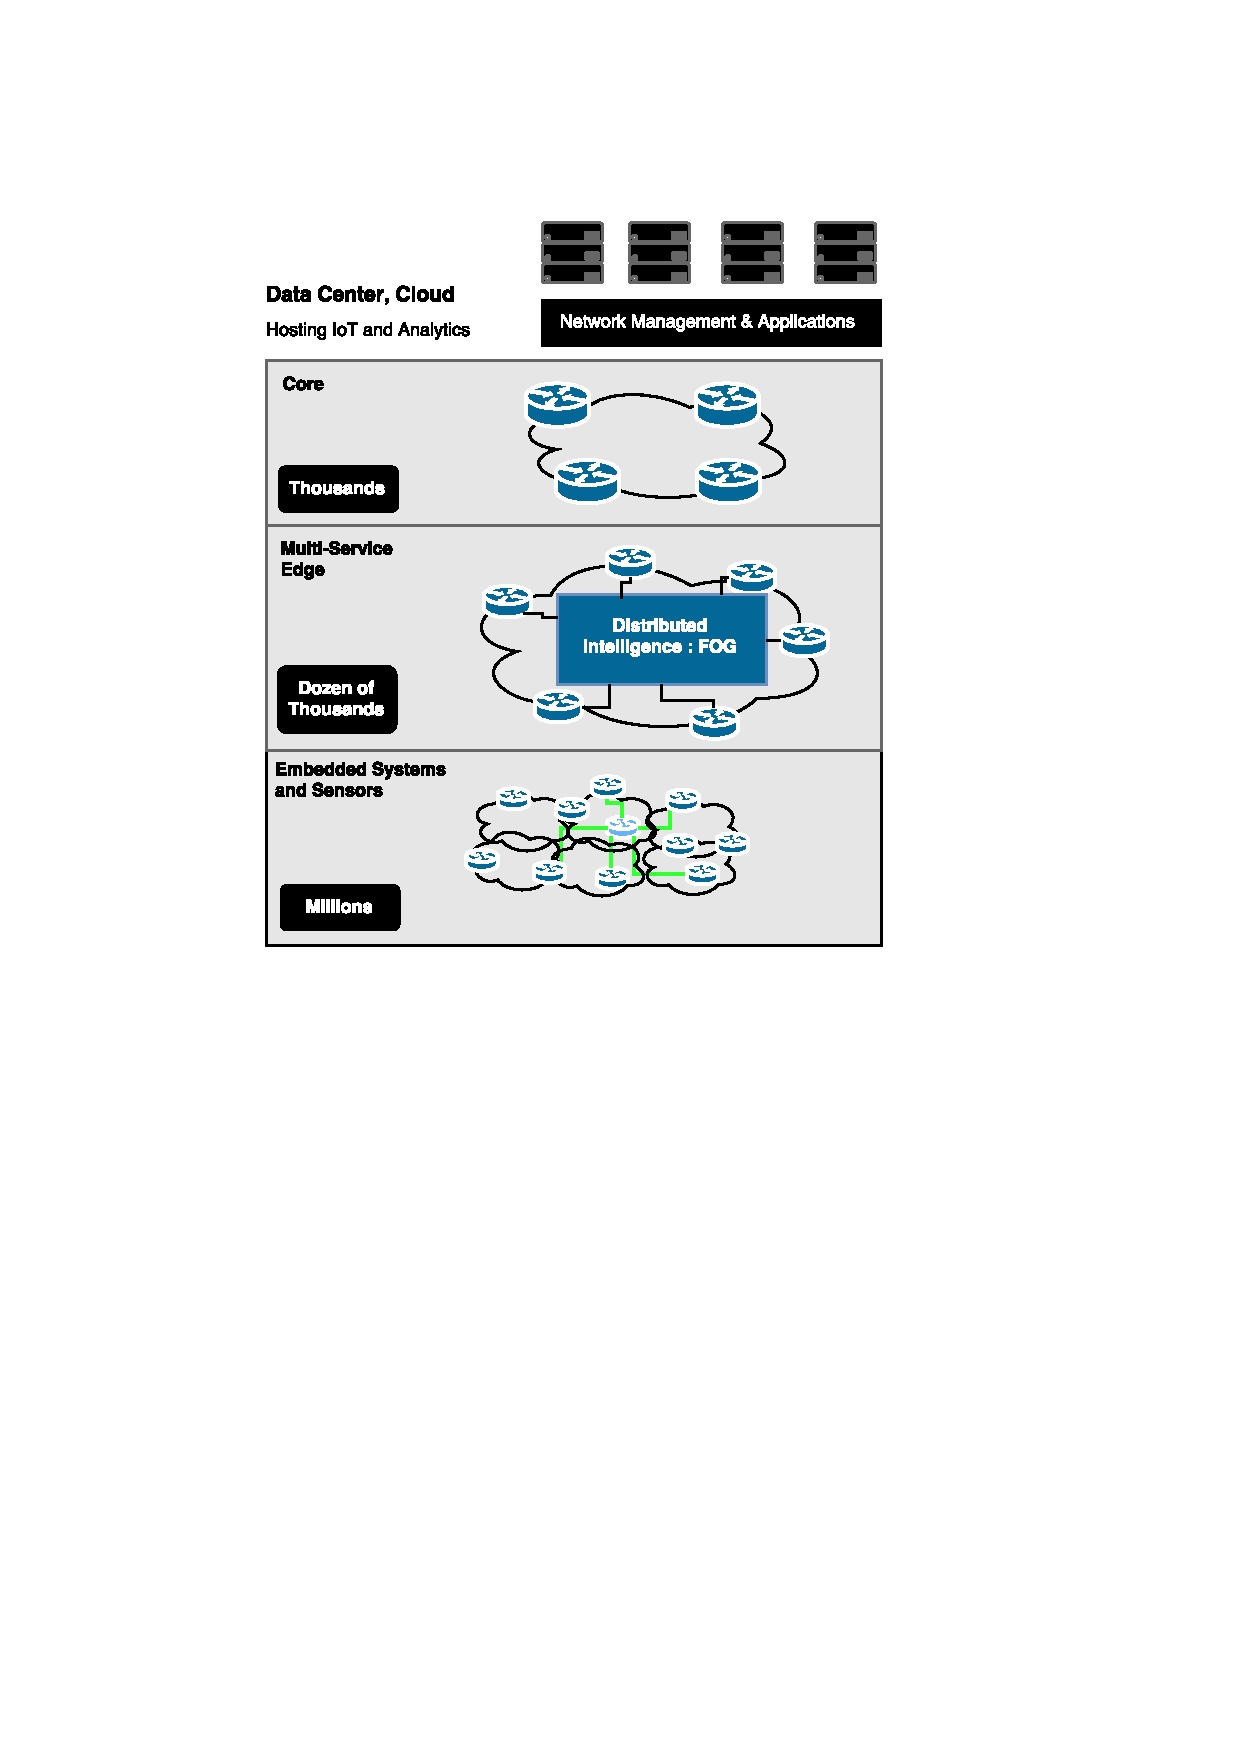
\includegraphics[width=.9\textwidth]{./images/fog_architecture}
  \caption{The Internet of Things and Fog Computing (Bonomi et. al (2012)).}
  \label{fig:fog_architecture}
\end{figure}

Figure~\ref{fig:fog_architecture} presents the architecture of the Fog Computing platform.
The distributed infrastructure of the Fog is composed of heterogeneous resources that must be managed
in a distributed way. The infrastructure comprising of several players, covering from data centers,
core of the network, edge of the network and end devices. The \textit{Embedded Systems and Sensors} is
the lowest layer of the Fog and it is responsible to perform \gls{M2M} interaction. It collects and
process the data from the sensors, issues controls to the actuators and also filters the data that
is locally consumed and send the rest to the higher layers. The \textit{Multi-Service Edge} and
\textit{Core} layers are responsible to perform visualization and reporting - e.g. \gls{H2M} interaction -
as well to deal with systems and processes (\gls{M2M}).\\

Since that interaction between the different layers can range from seconds - e.g. low-latency real-time
analytics - to days - transactional analytics - the Fog must support several types of storage, from
ephemeral storage at the lowest layers to semi-permanent at the highest layer. It is important to point
that the higher the tier, the geographical coverage is wider and the time scale is larger \cite{bonomi2014fog}.
The global coverage is given by the Cloud, which acts as a central repository for the persistent data
and that is used to perform business analytics.

\subsection{RFID Middleware}
\label{sub:rfid_middleware}
The \gls{RFID} middleware is the component of a \gls{RFID} system that sits between the low level
components - e.g. readers and tags - and the business client application - e.g. \gls{ERP} systems.
The next paragraphs describes the EPCglobal, a framework that provides standardized interfaces that
isolates hardware vendors from business applications, and Fosstrak, a open-source \gls{RFID}
middleware platform that implements the GS1 \gls{EPC} Network standards.

% GS1 EPC Network
\subparagraph{GS1 EPCglobal Architecture}
\label{subp:epc_network}
GS1\footnote{http://www.gs1.org} is an organization that is responsible for the development and maintenance of standards for
supply chain. One of the standards developed by GS1 is the \gls{EPC}, which is a unique serial identifier
for \gls{RFID} tags. GS1's subsidiary EPCglobal Inc.\footnote{http://www.gs1.org/epcglobal} created
the EPCglobal Architecture Framework, that currently is the standard for \gls{RFID} platforms.
Figure~\ref{fig:epc_architecture} presents the a high-level architecture of the EPCglobal framework
that shows its main interfaces and roles.\\

% EPC Architecture
\begin{figure}[ht!]
  \centering
  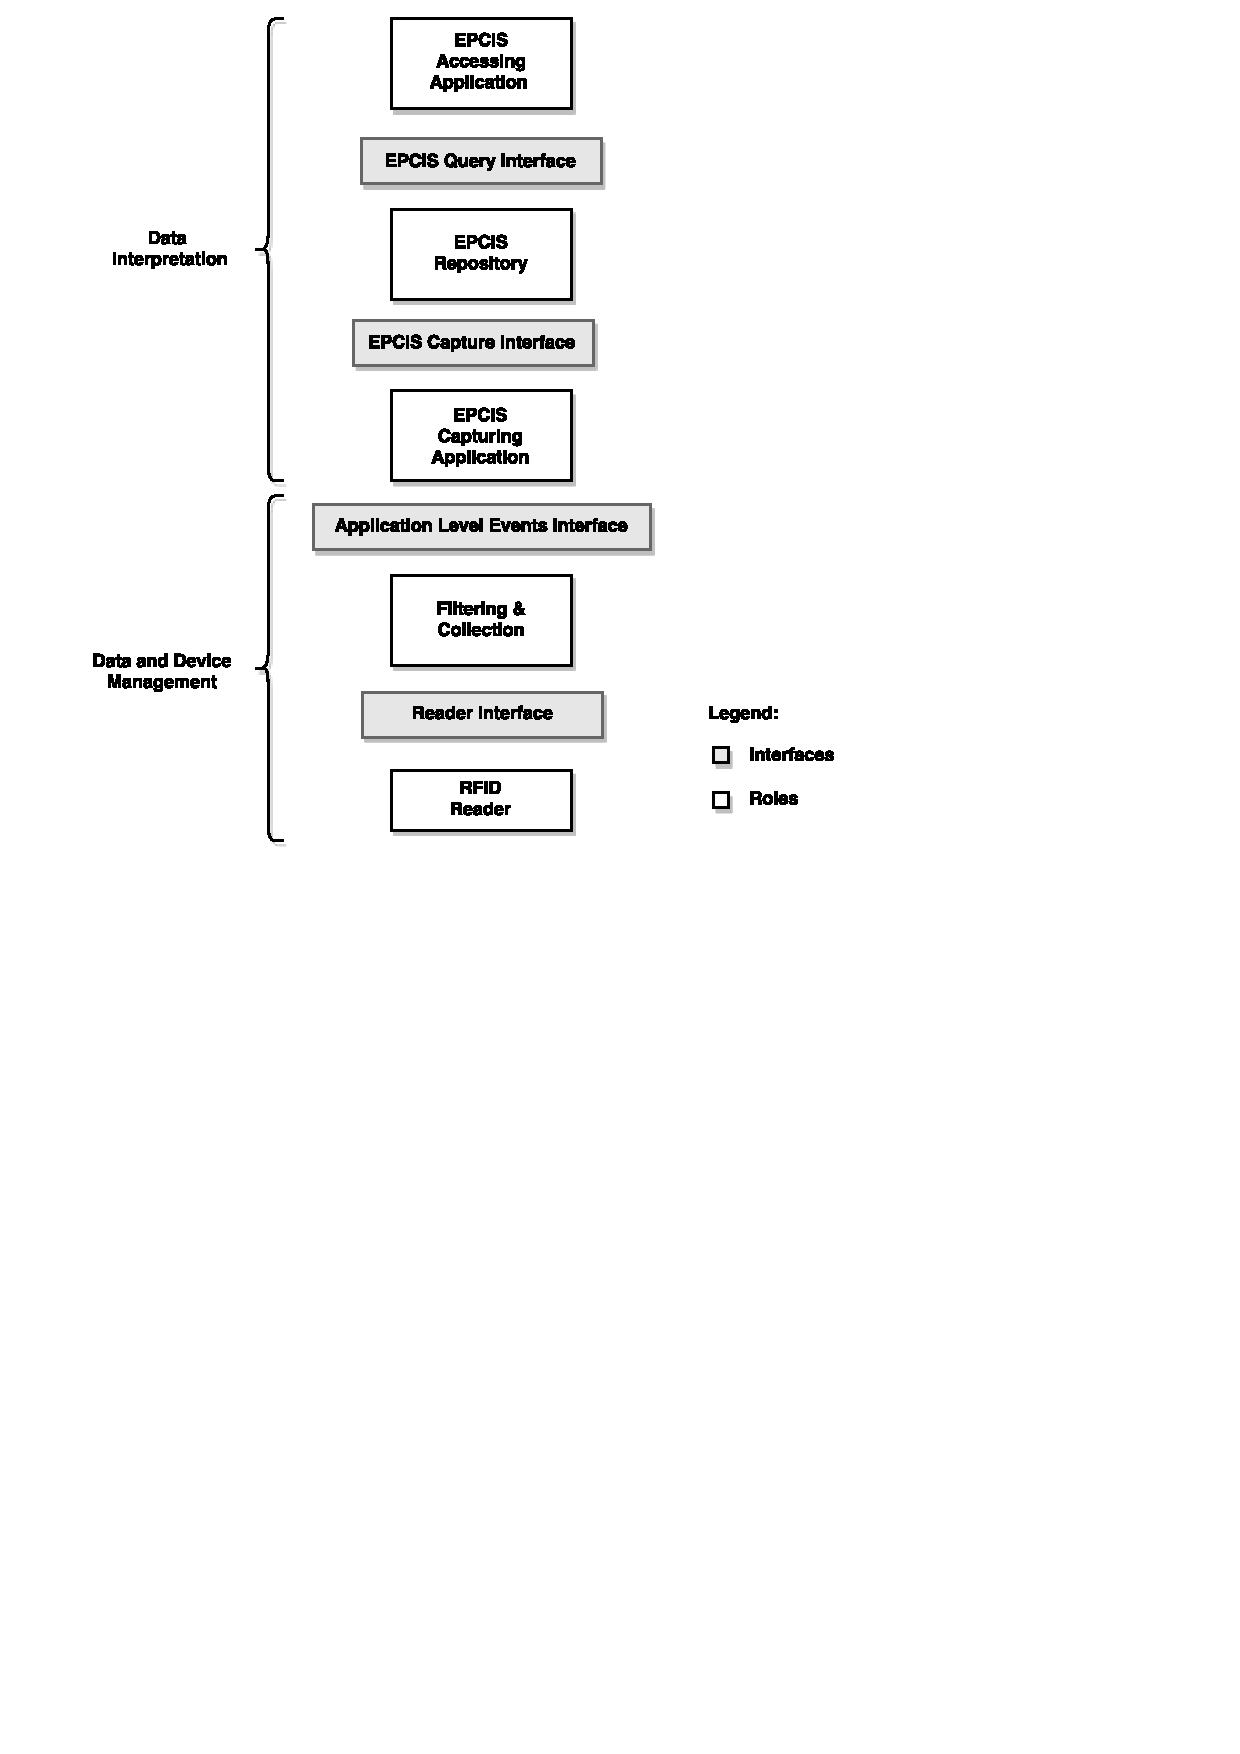
\includegraphics[width=.8\textwidth]{./images/EPCGlobal_architecture}
  \caption{GS1 EPCGlobal Architecture Framework.}
  \label{fig:epc_architecture}
\end{figure}

The framework\footnote{For more information about the EPCglobal Framework Architecture standard, the
full documentation is available at \href{http://www.gs1.org/gs1-architecture}{GS1 standards}} has a
set of standardized interfaces that enables the interchange of information between entities. In the
context of our work, the most relevant components of framework architecture are:

% EPC Architecture components
\begin{itemize}
  % Reader Interface
  \item Reader Interface provides the interfaces that must be implemented by the \gls{RFID} readers.
  The \gls{LLRP} standard provides interfaces that allows to control all the aspects of \gls{RFID}
  reader operation.
  % Filtering & Collection
  \item Filtering \& Collection is the module that coordinates the \gls{RFID} readers that are in the
  same physical space and also abstracts the readers from the upper layers. It allow to execute read
  and write operations on tags. Furthermore, it is responsible to filter, aggregate and grouping the
  raw tag data when requested.
  % Filtering & Collection Interface
  \item \gls{ALE} Interface defines the control and delivery of filtered and collected data from the
  Filtering \&  Collection to the \gls{EPCIS} Capturing Application. The \gls{ALE} are a selection of
  the events that are meaningful for the client applications.
  % EPCIS Capture Application
  \item EPCIS Capture Application supervises the operation of the lower EPC layers, and provides
  business context based on information involved in the execution of a particular step of a business
  process.
  % EPCIS Repository
  \item EPCIS Repository is the module where all the business events generated by EPCIS Capturing
  Applications are stored to be later be accessed by EPCIS Accessing Application. The EPCIS Query
  Interface defines how client applications can retrieve information from the repository.
\end{itemize}

% Fosstrak
\subsection{Fosstrak Platform}
\label{sub:fosstrak}
The Free and Open Source Software for Track and Trace (Fosstrak) is an EPCglobal Network compliant
\gls{RFID} software platform that was developed by Floerkemeier et. al \cite{floerkemeier2007rfid}.
Figure~\ref{fig:fosstrak_architecture} presents the architecture of the Fosstrak platform.

% Fosstrak Architecture
\begin{figure}[ht!]
  \centering
  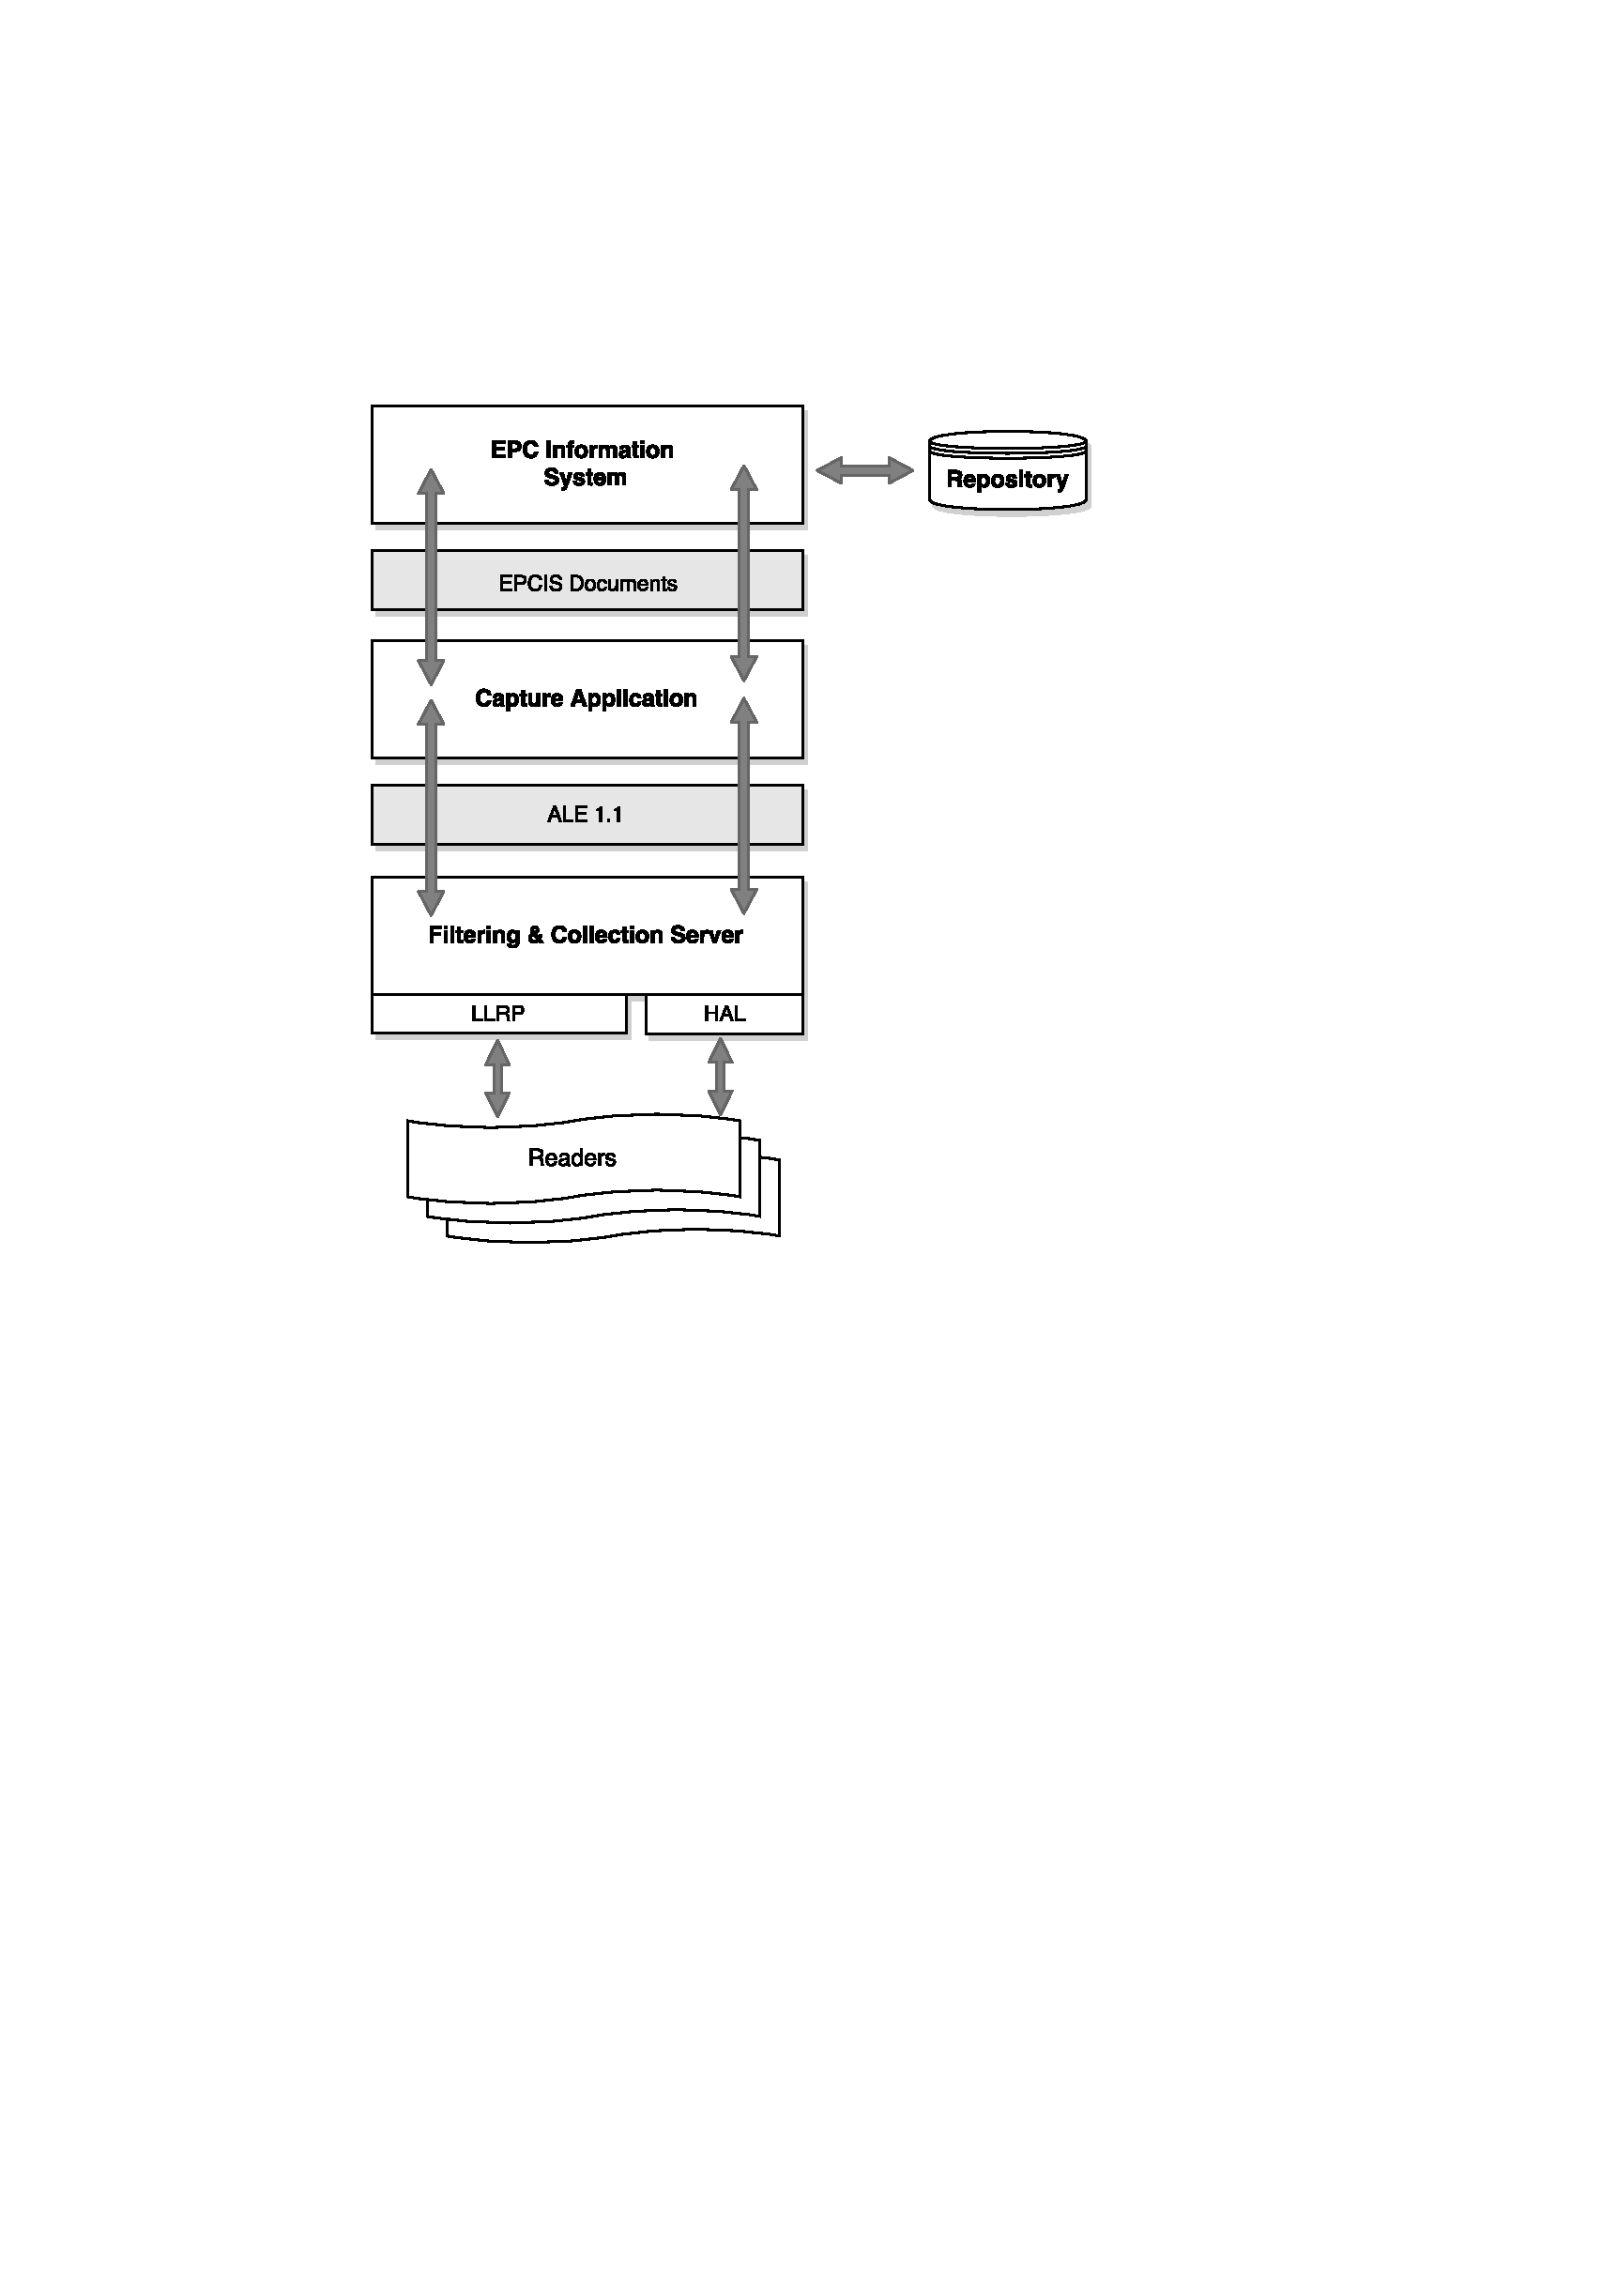
\includegraphics[width=.725\textwidth]{./images/fosstrak_architecture}
  \caption{Fosstrak architecture.}
  \label{fig:fosstrak_architecture}
\end{figure}

The Fosstrak platform is composed of three modules that implements the corresponding roles in the
\gls{EPC} Network: \textit{Reader Module}, \textit{Filtering and Collection Middleware Module} and
\textit{EPCIS Module}. For our work the relevant modules of the platform are:

% Fosstrak Modules
\begin{itemize}
  % FCServer
  \item \textit{Filtering \& Collection Server} is the module responsible to filter and collect data
  from \gls{RFID} readers. To communicate with readers, the module uses the \gls{LLRP} standard to
  for \gls{LLRP} compliant readers and uses the Fosstrak \gls{HAL} for unsupported readers. The
  module internally abstracts the readers as LogicalReaders instances, that are defined and configured
  through a \textit{LRSpec} document as defined by EPCglobal. Fosstrak also implements the
  \textit{Event Cycle}, that is the interval of time during which tags are read. The output of
  an \textit{Event Cycle} is the ECReport document that is sent to the Capturing Application.
  % Capturing Application
  \item \textit{Capturing Application} is part of the EPCIS module. This module is responsible to
  transform the uninterpreted events received on the ECReports into meaningful business events.
  Regarding its implementation, the Capturing Application is built on top of the Drools\footnote{http://www.drools.org/}
  engine where rules can be specified in the form of: ``when'' something happens, ``then'' do ``this''.
  Unfortunately, the rules are static and ones defined they can not be updated in runtime if needed.
  \item \textit{EPCIS Repository} provides an EPCglobal-certified EPCIS Repository. This means that
  all Fosstrak EPCIS modules and interfaces are compliant with the EPCglobal standard. The module
  provides persistence for \gls{EPCIS} events. To store new events the module provides the
  \textit{capture interface} and to retrieve historical events the module provides the \textit{query
  interface}. The module provides two EPC Network-conformant interfaces to a relational database
  (currently MySQL).
\end{itemize}

% Containers
\subsection{Containers}
\label{sub:containers}
Containers are a virtualization technique that is performed at \gls{OS} level, different of
hypervisor-based solutions - e.g. \glspl{VM} - where the virtualization is performed at hardware-level.
In a \gls{OS} level virtualization, all guests share the same operating system as the base machine \cite{matthews2007quantifying}.
While the effect of both types of virtualization are similar, unlike the hypervisor-based virtualization
an \gls{OS} level virtualization does not provide the ability to run multiple \glspl{VM} with different
operating systems on the same physical machine. However, \gls{OS} level virtualization provides significant
benefits when compared to hypervisor-based solutions. Containers are small, they have low memory and
\gls{CPU} overhead, they also are portable between different virtualization environments \cite{soltesz2007container}.\\

Docker\footnote{https://www.docker.com/} is an open source project to pack, ship and run any application as
a lightweight container. Docker is based on \gls{LXC}, which are hardware-agnostic and platform-agnostic,
this means that these containers can run anywhere\footnote{Initially, Docker required that the physical
machine where the containers will be created was running a Linux kernel. However, recently Microsoft
launched Windows Server Containers, a \gls{OS} level virtualization mechanism where is possible to
perform the management of containers through Docker.}, from a laptop to a cloud instance. Another
benefit that Docker platform provides is the Docker Hub\footnote{https://hub.docker.com/} service,
a public repository that stores Docker images used to create the containers.

% Configuration Management Tools
\subsection{Configuration Management Tools}
\label{sub:cm_tools}
\gls{CM} tools are software management tools are software tools that allows to automate and specify
the deployment of an application. Usually, users describes the system resources and their desired
state and the \gls{CM} tool is responsible to enforce the state specified by the user.
For instance, \gls{CM} tools allows to automate the provisioning of physical and virtual machines,
perform dependency management of software components and to configure management tasks.\\

Currently, there are several solutions to perform configuration management of software, where the
most relevant are Chef\footnote{https://www.chef.io/}, Puppet\footnote{https://puppetlabs.com/},
Ansible\footnote{http://www.ansible.com/} and Salt\footnote{http://saltstack.com/}. The main difference
between these tools is that some of the them are oriented to developers, which is the of Chef and Puppet
that requires some programming to be used, while others are oriented to system administrators, which
is the case of Ansible and Salt.

% ------------------------------------------
%   INFORMATION AND SOFTWARE ENGINEERING
% ------------------------------------------
%  CLOUD4THINGS MASTER THESIS DISSERTATION
% ------------------------------------------
% Author: Marcus Vinicius Paulino Gomes
%
% Advisors:
% - Dr. Miguel Filipe Leitão Pardal
% - Dr. José Manuel da Costa Alves Marques
% ------------------------------------------
\documentclass[10pt,twoside,a4paper]{report}
% Set document margins to 1in in all sides
\usepackage[margin=2.5cm]{geometry}
% Line spacing package
\usepackage{graphicx, helvet, inputenc, setspace}
% Set main font to Arial
\renewcommand{\familydefault}{\sfdefault}
% Page numbering
\pagestyle{plain}
% ------------------------------------------
%  CLOUD4THINGS MASTER THESIS DISSERTATION
% ------------------------------------------
% Set line spacing to 1.5cm
\onehalfspacing
\begin{document}
%!TEX root = ./dissertation.tex

% ---------------------------------------------------------
%   MASTER THESIS DISSERTATION COVER
% ---------------------------------------------------------
\begin{titlepage}
% ---------------------------------------------------------
%  INSTITUTION LOGO
% ---------------------------------------------------------

\includegraphics[width=5cm]{images/ist_logo}~\\
%
\if\IsFinalVersion 1
  \vspace*{\finalLogoSpacing}
\else
  \vspace*{\draftLogoSpacing}
\fi

\begin{center}
% ---------------------------------------------------------
%  MASTER THESIS DISSERTATION TITLE
% ---------------------------------------------------------
{\LARGE \textbf{\Title}}\\[1.0cm]
% ---------------------------------------------------------
%  MASTER THESIS DISSERTATION SUBTITLE
% ---------------------------------------------------------
{\Large \Subtitle}\\[1.0cm]
% ---------------------------------------------------------
%  AUTHOR NAME (FULL)
% ---------------------------------------------------------
{\Large \textbf{\StudentName}}\\[1.0cm]
% ---------------------------------------------------------
%  DISSERTATION DEGREE
% -----------------------------------------------------------------
{\large Thesis to obtain the Master of Science Degree in}\\[1.0cm]
% -----------------------------------------------------------------
%  COURSE NAME
% -----------------------------------------------------------------
{\LARGE \textbf{\DegreeName}}\\[1.0cm]

% -----------------------------------------------------------------
%  ADVISORS NAME
% ---------------------------------------------------------
\begin{minipage}[t]{.4\textwidth}
  \center
  \begin{flushright}
    {\large Supervisors:~~}
  \end{flushright}
\end{minipage}%
\begin{minipage}[t]{.6\textwidth}
  \center
  \begin{flushleft}
    {\Supervisors}
  \end{flushleft}
\end{minipage}\\
%
\if\IsFinalVersion 1
  \vspace*{\finalAdvisorsSpacing}
\else
  \vspace*{\draftAdvisorsSpacing}
\fi
% ---------------------------------------------------------
%  JURI NAMES:
%  - PRESIDENT
%  - ADVISOR
%  - VOGALS
% ---------------------------------------------------------
\if\IsFinalVersion 1
%
\begin{minipage}[t]{1\textwidth}
  \center
  {\Large \textbf{Examination Committee}}\\[.25cm]
  {\large Chairperson: \Chairperson}\\
  {\large Supervisor: \MainSupervisor}\\
  {\large Member of the Committee: \CommitteeMembers}
\end{minipage}\\[1.0cm]
%
\fi

\if\IsFinalVersion 1
 \vspace*{\dateSpacing}
\fi

% ---------------------------------------------------------
%  DATE (MONTH AND YEAR)
% ---------------------------------------------------------
{\Large \textbf{\Month\:\Year}}\\
\end{center}
\end{titlepage}

\begin{abstract}
In this document we present Cloud4Things, a solution that proposes to make the deploy and manage IoT applications for smart places.
Due to the heterogeneity of IoT applications, management tasks such as application deployment and management are complex tasks
that require advanced technical knowledge. Cloud4Things proposes to decrease the complexity of these tasks by adopting a high-level perspective
enables to perform the deployment and management operations of IoT applications.
To simplify the deployment operation at the Cloud, Cloud4Things will rely on cloud orchestrators tools to execute such task.
These orchestration tools allow the specification of the application structure in high-level abstraction and allow the control the life-cycle of the application.
Cloud4Things will allow the management of the provisioned resources at the Cloud by a smart place only having in mind
the business rules of this particular space. With Cloud4Things, smart places managers will be able to monitor the performance of its
smart place in real time. This document also presents the state-of-the-art solution as well an overview about the proposed approaches and
evaluation methods.
\keywords{Internet of Things, Cloud Computing, Smart Places, Service Level Agreements, Orchestration Tools, Automated Deployment}
\end{abstract}

\end{document}

\section{Evaluation Methodology}
\label{sec:evaluation}
The evaluation of the solution will be performed according to two perspectives: one consists in
evaluating the performance of the Cloud and the other consists in evaluate the performance
of the deployment of the application.
% -------------------------------------
%  APPLICATION DEPLOYMENT EVALUATION
% -------------------------------------
\subsection{Application Deployment Evaluation}
\label{sub:application_deployment_evaluation}
The performance of the application deployment is an important aspect to be evaluated.
The deployment operation can be evaluated in terms of the metrics of \textit{Network Bandwith},
\textit{Data Volume} and \textit{Latency} of the process. These values determine
the efficiency of the deployment operation. For instance, if we have a high \textit{Data Volume}
and a low \textit{Network Bandwith} available, the \textit{Latency} of the deployment process
will present high values.     
% -------------------------------------
%  CLOUD PERFORMANCE EVALUATION
% -------------------------------------
\subsection{Cloud Performance Evaluation}
\label{subs:cloud_performance_evaluation}
An aspect that is important concerns with the performance of the Cloud regarding the amount
of data generated by the events. Cloud computing creates an illusion that available computing
resources on demand are limitless \cite{armbrust2009m}. However, with the increase of the amount of
events, we must measure these computing resources in order to determine if the system is fulfilling
the \textit{QoS} requirements. To perform the evaluation of the behaviour and performance of the Cloud
we need to measure some system metrics such as:
\begin{itemize}
  \item \textit{CPU Utilization:} indicates the percentage of time that the CPU was working at
  the instances in the Cloud. Normally, this metric is available through the Cloud providers.
  Usually, the range of this metrics is given in percentage that can vary between 0-100\%.
  \item \textit{Memory Usage:} indicates the amount of memory that is consumed by the system in a
  given period of time. The unit of this metric is given in MBytes.
  \item \textit{System Load:} is a metric that indicates the general state of the system.
  This metric estimates the general performance of the system by measuring the number of received events.
  The range of this metric varies between 0 and 1. When this metric has a value of 0, it means that the
  system is not receiving any events at the time. If this metric has a value of 1, it means that the system
  is overloaded, consequently the CPU Utilization and Memory Usage metrics are close to the maximum value.
\end{itemize}

%!TEX root = ../dissertation.tex

\chapter{Experiment Results}
\label{chapter:results}
Evaluation here...

%!TEX root = ../dissertation.tex

\chapter{Evaluation}
\label{chapter:evaluation}
% 1. Present an overview of the evaluation, what we want to evaluate, what we want to conclude.
The present chapter describes the evaluation methodology as also the experiments performed to determine
if a cloud-based approach is adequate to host \gls{RFID} applications middleware. The evaluation process
will focus on establish if such approach can met the low-latency and scalable data storage requirements
for those applications.\\

Our main goal is to obtain statistical values that allow us to assert if a cloud-based approach is able
to fulfill the expected requirements. With these results, we want to specify which domains can rely in such
approach.

% 2. Present the evaluation methodology for both cases
\section{Evaluation Methodology}
\label{sec:eval_methodology}
In order to determine if a cloud-based \gls{RFID} application is able to met the latency and data
storage scalability requirements, we propose the following methodologies to perform the evaluation:

% Evaluation Methodologies : Data Storage
\subsection{Data Storage Scalability}
\label{sub:eval_methodology_data}
To evaluate the data storage scalability for a \gls{RFID} application based on Fosstrak, the proposed
methodology consists in stress the \gls{EPCIS} Repository by simulating several users that are
concurrently sending events - through \gls{HTTP} requests - to the \gls{EPCIS} repository that is
running in the cloud, as illustrated in Figure~\ref{fig:eval_data_methodology}. The cloud server is
running a monitoring system that periodically stores data related to a set of system metrics,
such as \textit{CPU Utilization} and \textit{Network Traffic}.\\

% Data Storage Evaluation Methodology Figure
\begin{figure}[ht!]
  \centering
  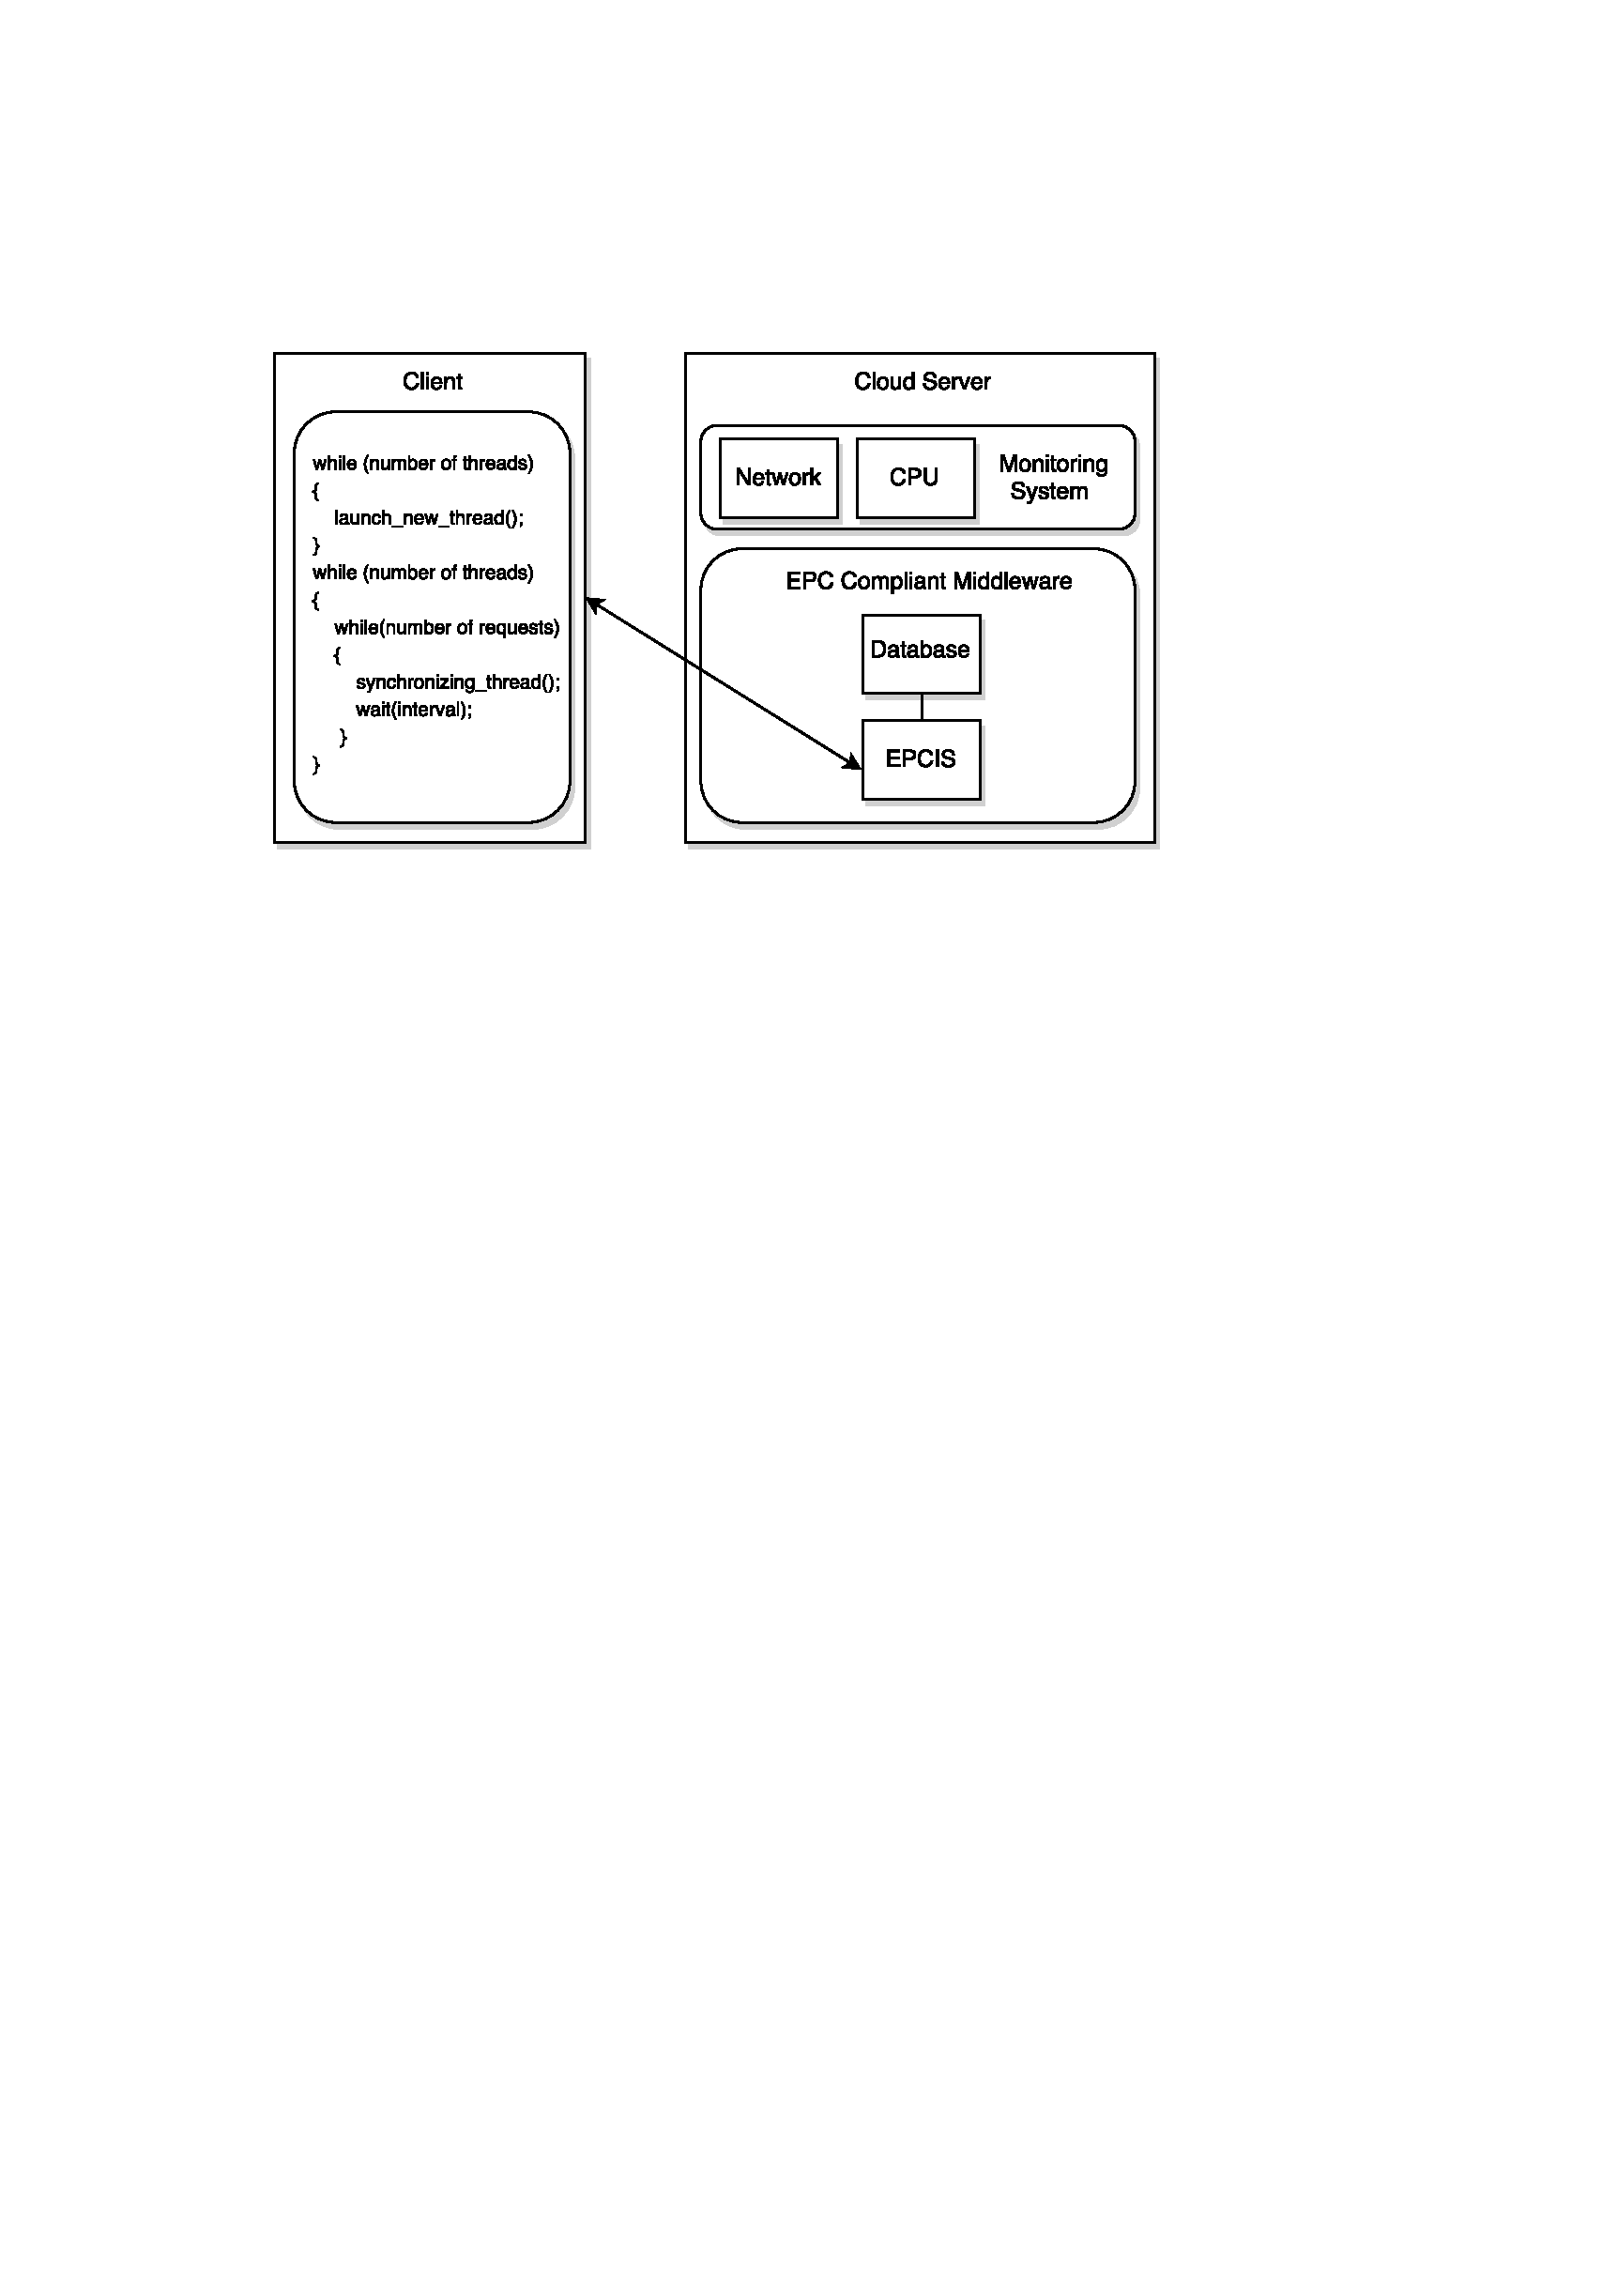
\includegraphics[width=.7\textwidth]{./images/eval_data_methodology}
  \caption{Data scalability evaluation methodology.}
  \label{fig:eval_data_methodology}
\end{figure}

The analysis of these metrics allows to observe how the performance and behavior of the \gls{EPCIS}
module is affected regarding the amount of events that are processed.

% Evaluation Methodologies : Latency
\subsection{Latency Interaction}
\label{sub:eval_methodology_latency}
To evaluate the response time between an event that occurs in the smart place and the corresponding
action that is triggered in the smart place, according the proposed methodology in Figure~\ref{fig:eval_latency_methodology}.\\

% Latency Interaction Evaluation Methodology Figure
\begin{figure}[ht!]
  \centering
  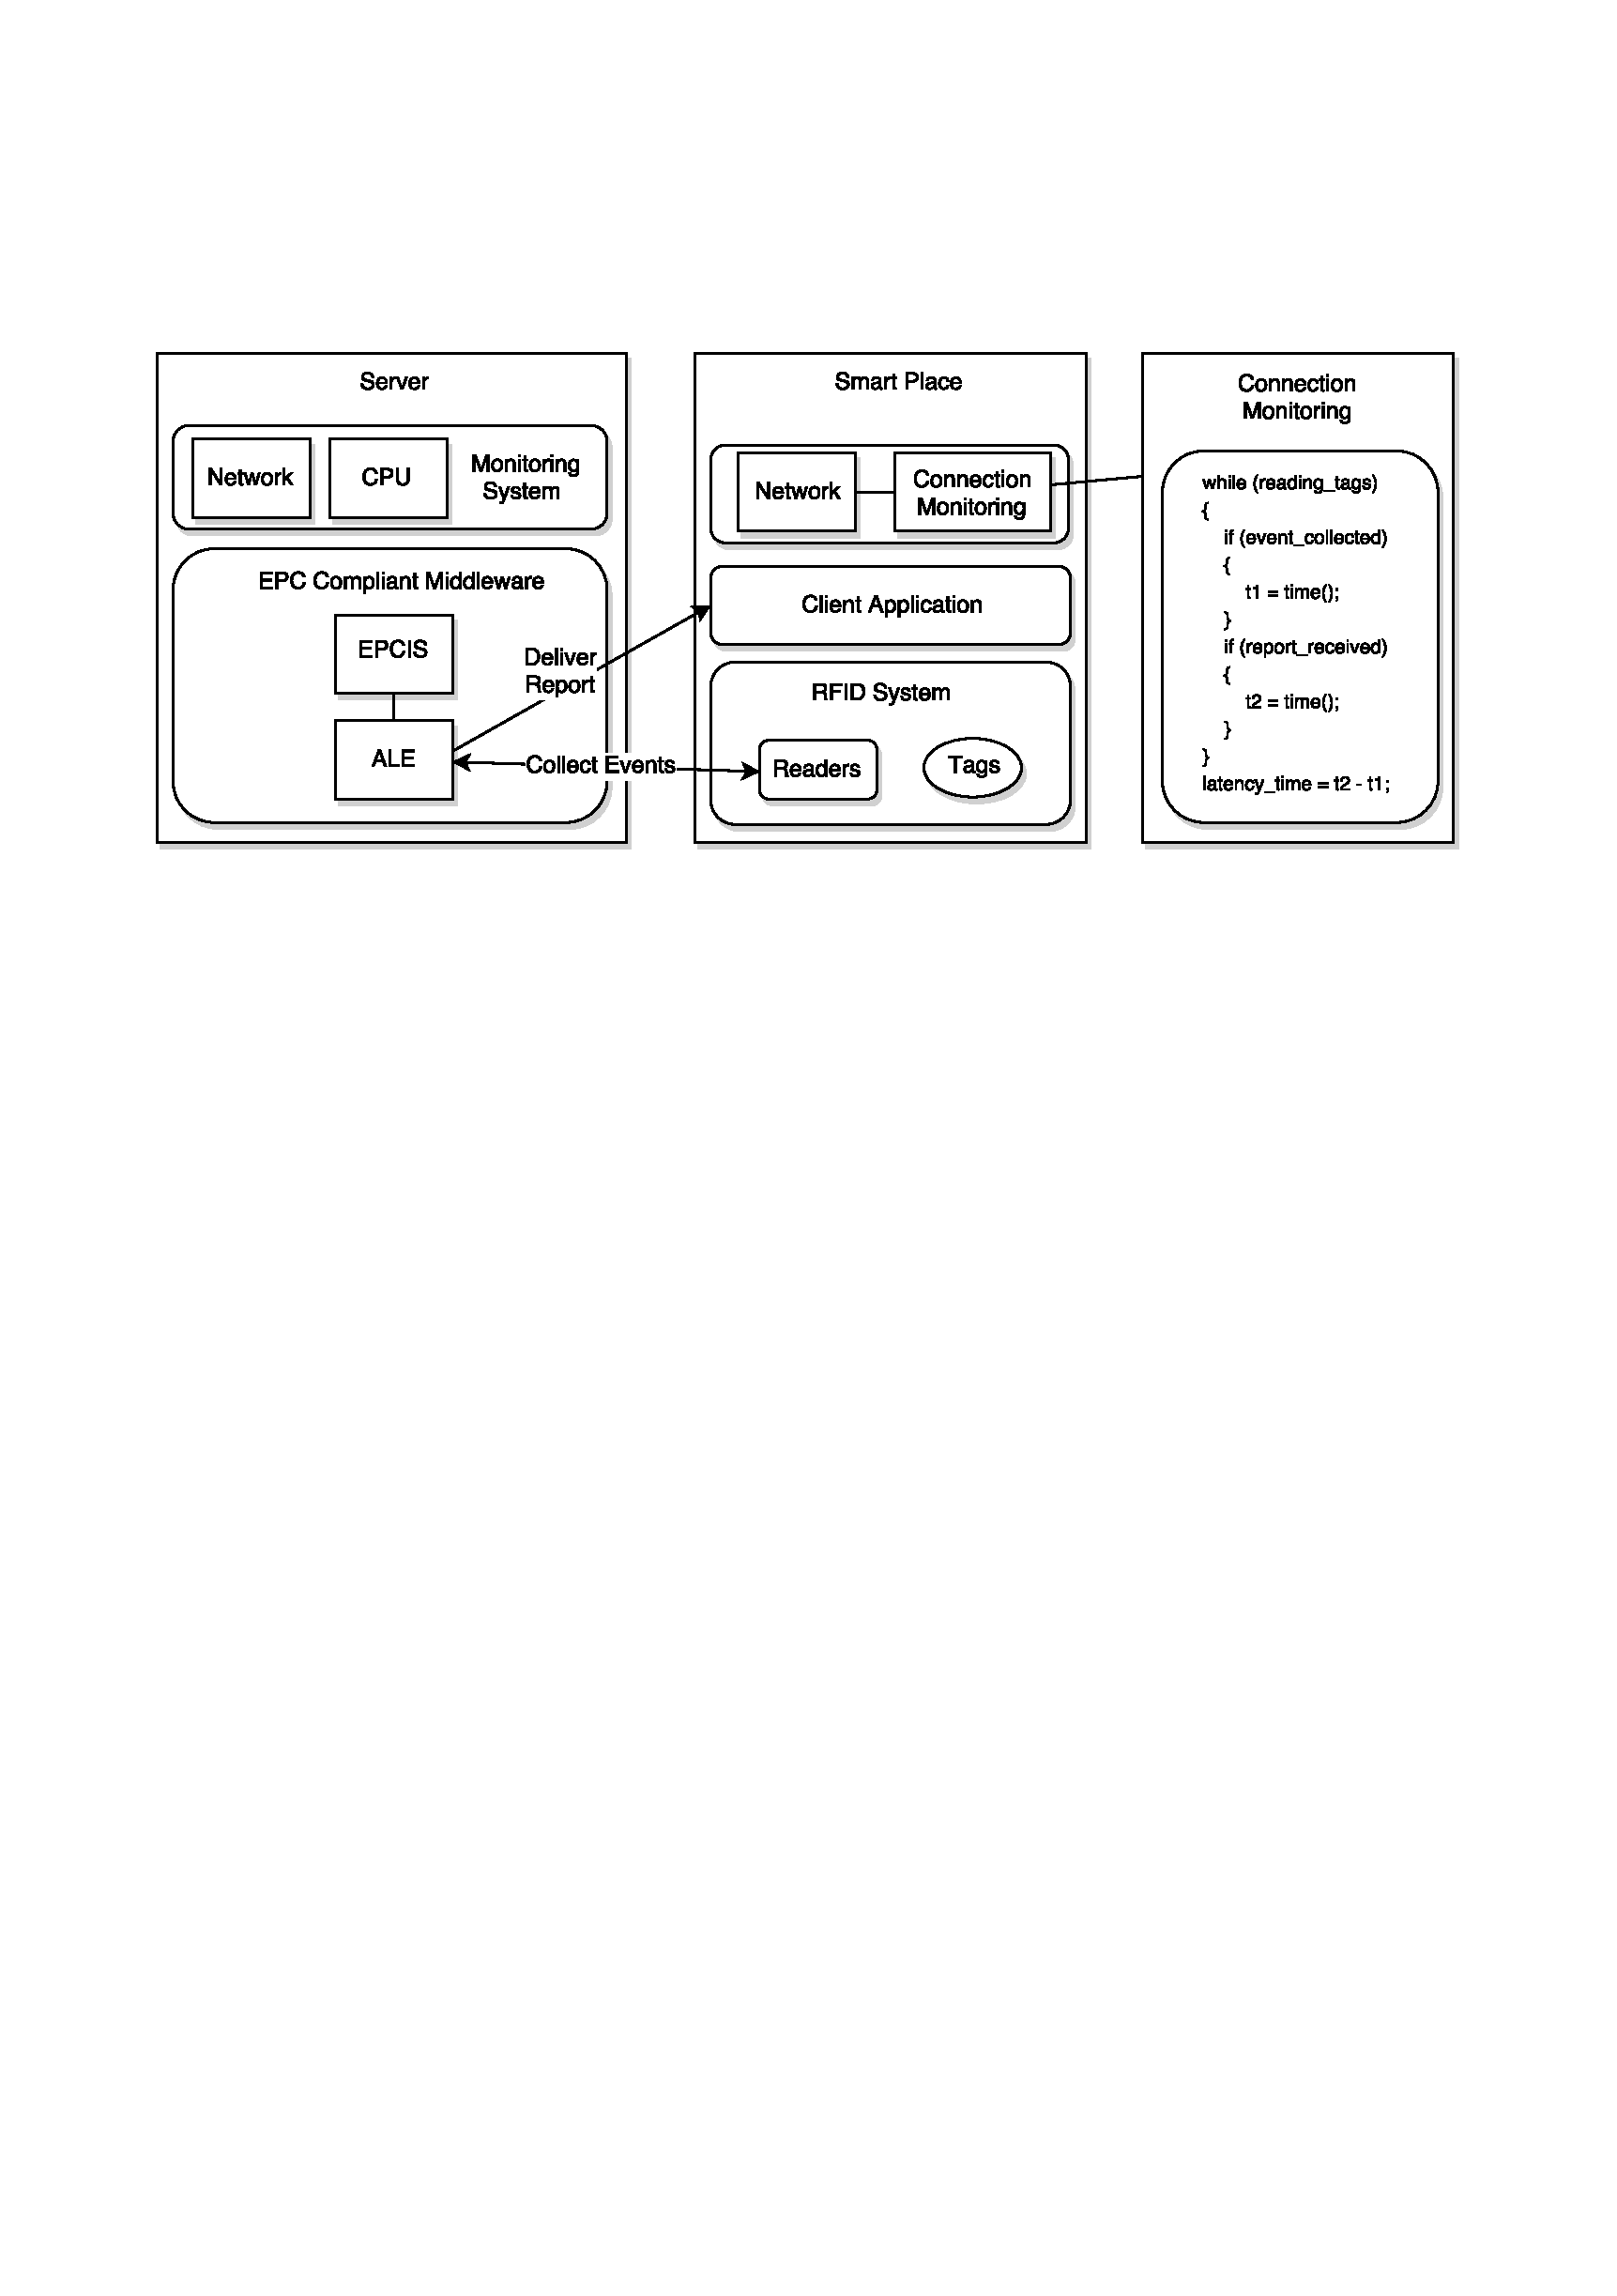
\includegraphics[width=.9\textwidth]{./images/eval_latency_methodology}
  \caption{Latency interaction evaluation methodology.}
  \label{fig:eval_latency_methodology}
\end{figure}

The \gls{ALE} module is responsible to collect and process the reader events and take the
correct decisions based on those events. In the Fosstrak implementation the collection and processing
of reader events is performed according to an \textit{Event Cycle} specification. The \textit{Event Cycle}
is a set of periodical read cycles where the \gls{ALE} module collect the events from readers. The data
about the \textit{Event Cycle} is delivered to the client through a report. The information in the report
can be used to notify the client regarding a situation in the smart place or even to trigger a new event
in the smart place such as open or close a door.\\

The smart place is running a monitoring system that stores information about the incoming and outgoing
connections. The Fosstrak \gls{ALE} module can be configured to generate information to register
when a new event is processed and also when a new reports is delivered to the client. Thus, with the
information provided by the monitoring system and the \gls{ALE} module it is possible to calculate
the latency request for an event that occurs in the smart place.\\

With this methodology we intend to obtain information regarding how the communication time is spent
when a event is triggered in the smart place the approaches described in \ref{sec:smart_place_architecture}.
In order to determine what approach is more adequate to host the application middleware, the proposed
metrics are considered:

% Metrics
\begin{itemize}
  \item \textit{Event Latency}: the time spent from the moment that an event is triggered in the
  smart place to the moment when the client application receives the notification of the event.
  \item \textit{Upload Latency}: the time spent from the moment that an event is triggered in the
  smart place from the moment when the \gls{ALE} module process the event.
  \item \textit{Processing Latency}: the time spent from the moment that the \gls{ALE} module process
  an event from the moment that the \textit{Event Cycle} report is created.
  \item \textit{Response Latency}: the time spent from the moment that the \gls{ALE} module delivers
  the \textit{Event Cycle} report to the moment that the client receives it.
\end{itemize}

The analysis of those metrics will allow us to compare the performance of both approaches and help to
determine which one is more adequate to host \gls{RFID} applications middleware.

% Evaluation Setup
\section{Evaluation Setup}
\label{sec:eval_setup}
To perform the evaluation experiments we choose \gls{AWS} as cloud provider. All the experiments were
conducted in \gls{AWS} \gls{EC2} instances running the Amazon Linux AMI operating system. The virtual
machines presents a configuration with a 2.5\textit{\gls{GHz}} single-core processor with 1\textit{\gls{GB}} of
\gls{RAM}. In the fog-aprroach configuration, where the \gls{ALE} module is provisioned in the smart place,
the experiments were conducted in a virtual machine with a 2.6\textit{\gls{GHz}} dual-core processor
with 2\textit{\gls{GB}} of \gls{RAM} and running the \textit{Linux Ubuntu 14.04.1 LTS} operating system.
Regarding the smart place infrastructure, the evaluation was performed through a \gls{ADSL} connection
and the Rifidi Emulator\footnote{http://rifidi.org} was used to emulate the physical readers that are
in the smart place.\\

Regarding software components, the application stack is composed of the \textit{Apache Tomcat 7.0.52.0}\footnote{http://tomcat.apache.org/}
with \textit{Java} version \textit{1.7.0} update \textit{79}. The \gls{RFID} middleware used was the Fosstrak
described in section \ref{sub:fosstrak}. The middleware stack is available at the Fosstrak's\footnote{http://fosstrak.github.io/}
source control system, and the versions were: a) \textit{FCServer} version \textit{1.2.0}; b) \textit{Capture Application}
version \textit{0.1.1}; and c) \textit{\gls{EPCIS} Repository} version \textit{0.5.0}. Furthermore,
the \gls{EPCIS} Repository was connected to a \textit{MySQL server} version \textit{5.5} that stores
all the \gls{EPCIS} events.

% Performed Experiments
\section{Experiments Performed}
\label{sec:eval_experiments}
The experiments performed in our evaluation were based on the scenario and data from the RFIDToys\cite{Correia:Thesis:2014}
Master Thesis.

\subsection{Data Scalability}
\label{sub:eval_exp_data}
To evaluate the data scalability for the Fosstrak middleware we use the data recorded with the Rec\&Play
- which is able to record \gls{RFID} sessions that stores the events occurred in the smart place
maintaining the order and time from the beginning of the session - module were used as base to execute
the tests.\\

As described in Section \ref{sub:eval_methodology_data}, the methodology consists in simulate a given
number of readers that are in the warehouse. The simulation was performed through Jmeter\footnote{http://jmeter.apache.org/},
a Java application designed to perform load testing and measure the application performance.
In order to reproduce some situations that can occur in a real smart place, we perform the following
variations in the tests:

% Test variations
\begin{itemize}
  \item\textbf{Standard} The test is executed with the amount of events and period from the recorded session.
  \item\textbf{Double of Requests} The test is executed with the period and twice of events from the recorded
  session.
  \item\textbf{Half of Interval} The test is executed with the amount of events and half of the period from
  the recorded session.
\end{itemize}

Each test case was executed simulating 5 readers at most in two scenarios, \textbf{Baseline} and
\textbf{Track 3 Laps}.

\subparagraph{Baseline}
\label{subp:eval_exp_data_baseline}
In the \textbf{Baseline} scenario the session contains the data recorded based in the events generated
during a 1 lap in the track. The parameters used to execute the test for this scenario are described in
Table~\ref{tab:baseline_parameters}.

% Baseline parameters
\begin{table}[ht!]
  \begin{tabular}{|c|c|}
    \hline
    Number of Events & Period \\ \hline
    1593             & 82ms   \\ \hline
  \end{tabular}
  \caption{Baseline evaluation parameters.}
  \label{tab:baseline_parameters}
\end{table}

% Baseline results
\begin{figure}[ht!]
\centering
\begin{subfigure}{.5\textwidth}
  \centering
  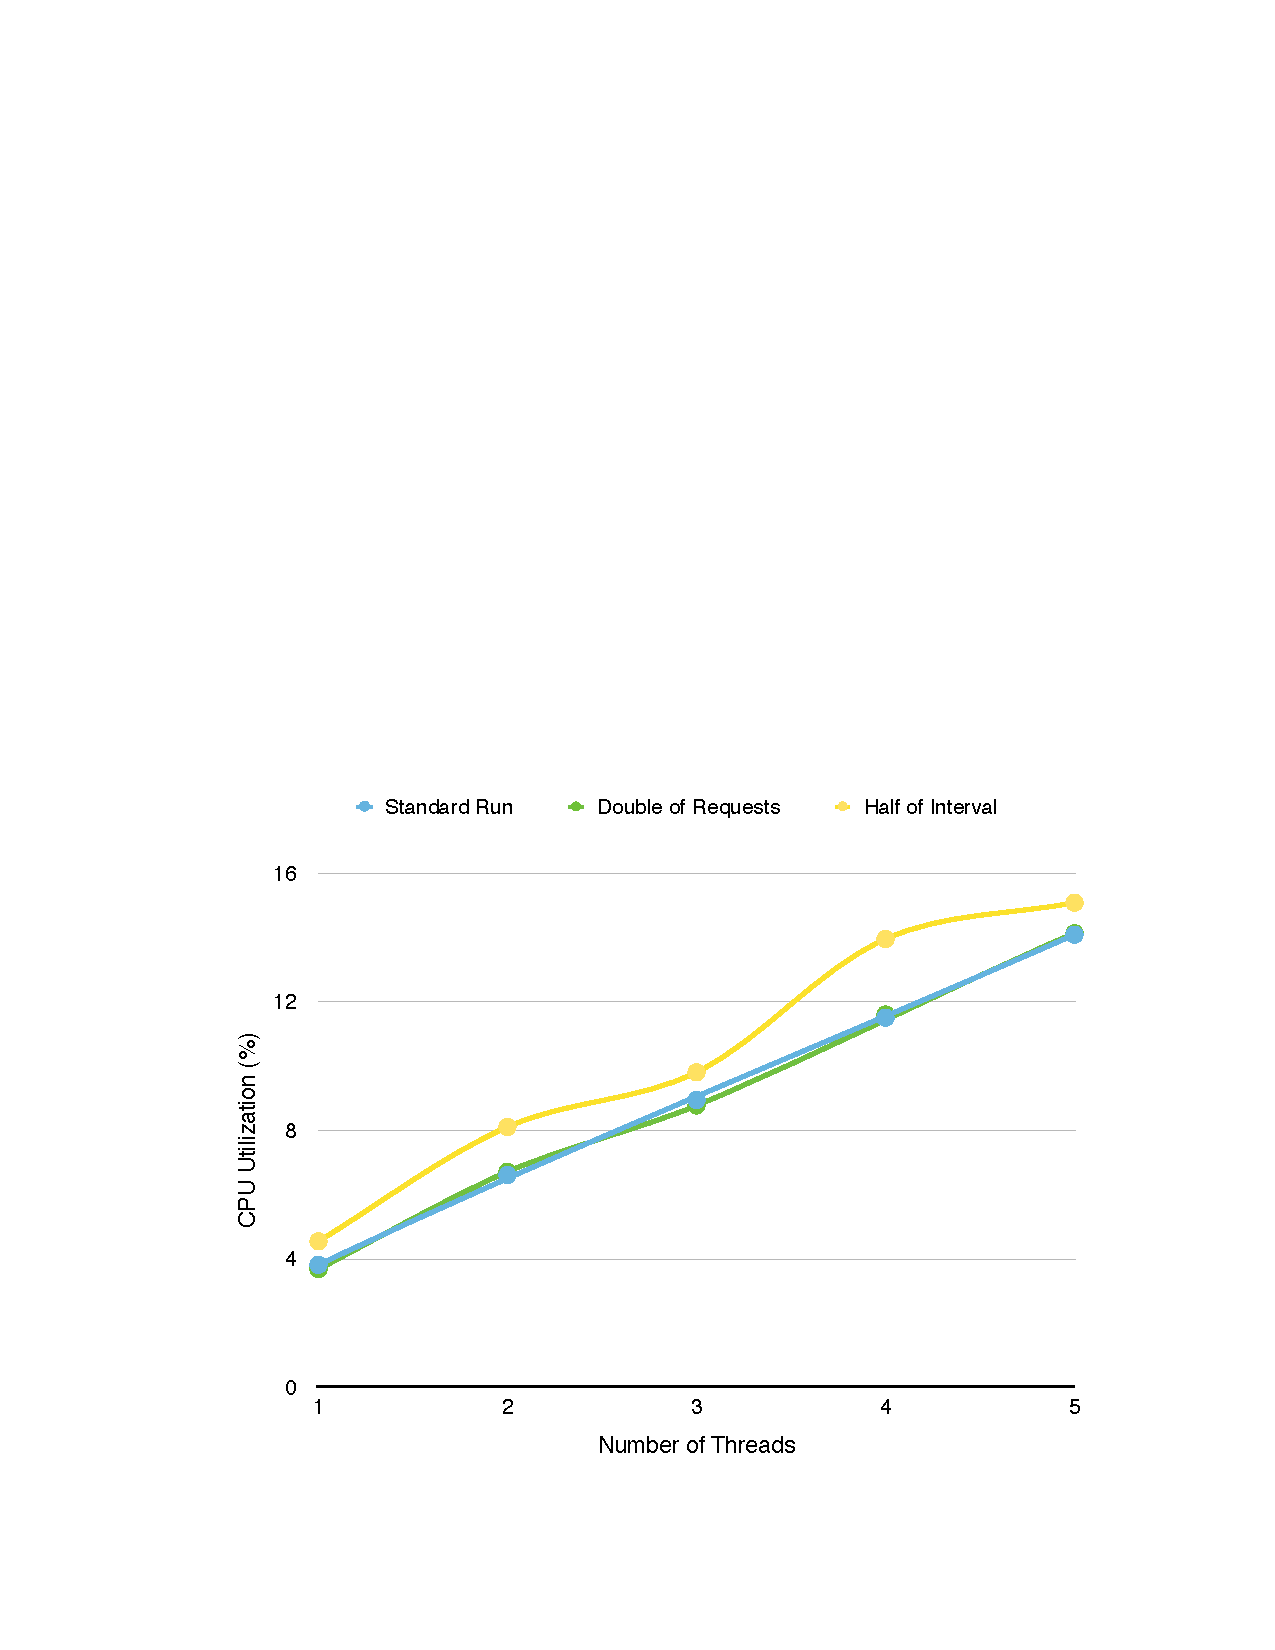
\includegraphics[width=\linewidth]{./images/cpu_1_lap}
  \caption{Baseline CPU Utilization.}
  \label{fig:eval_baseline_cpu}
\end{subfigure}%
\begin{subfigure}{.5\textwidth}
  \centering
  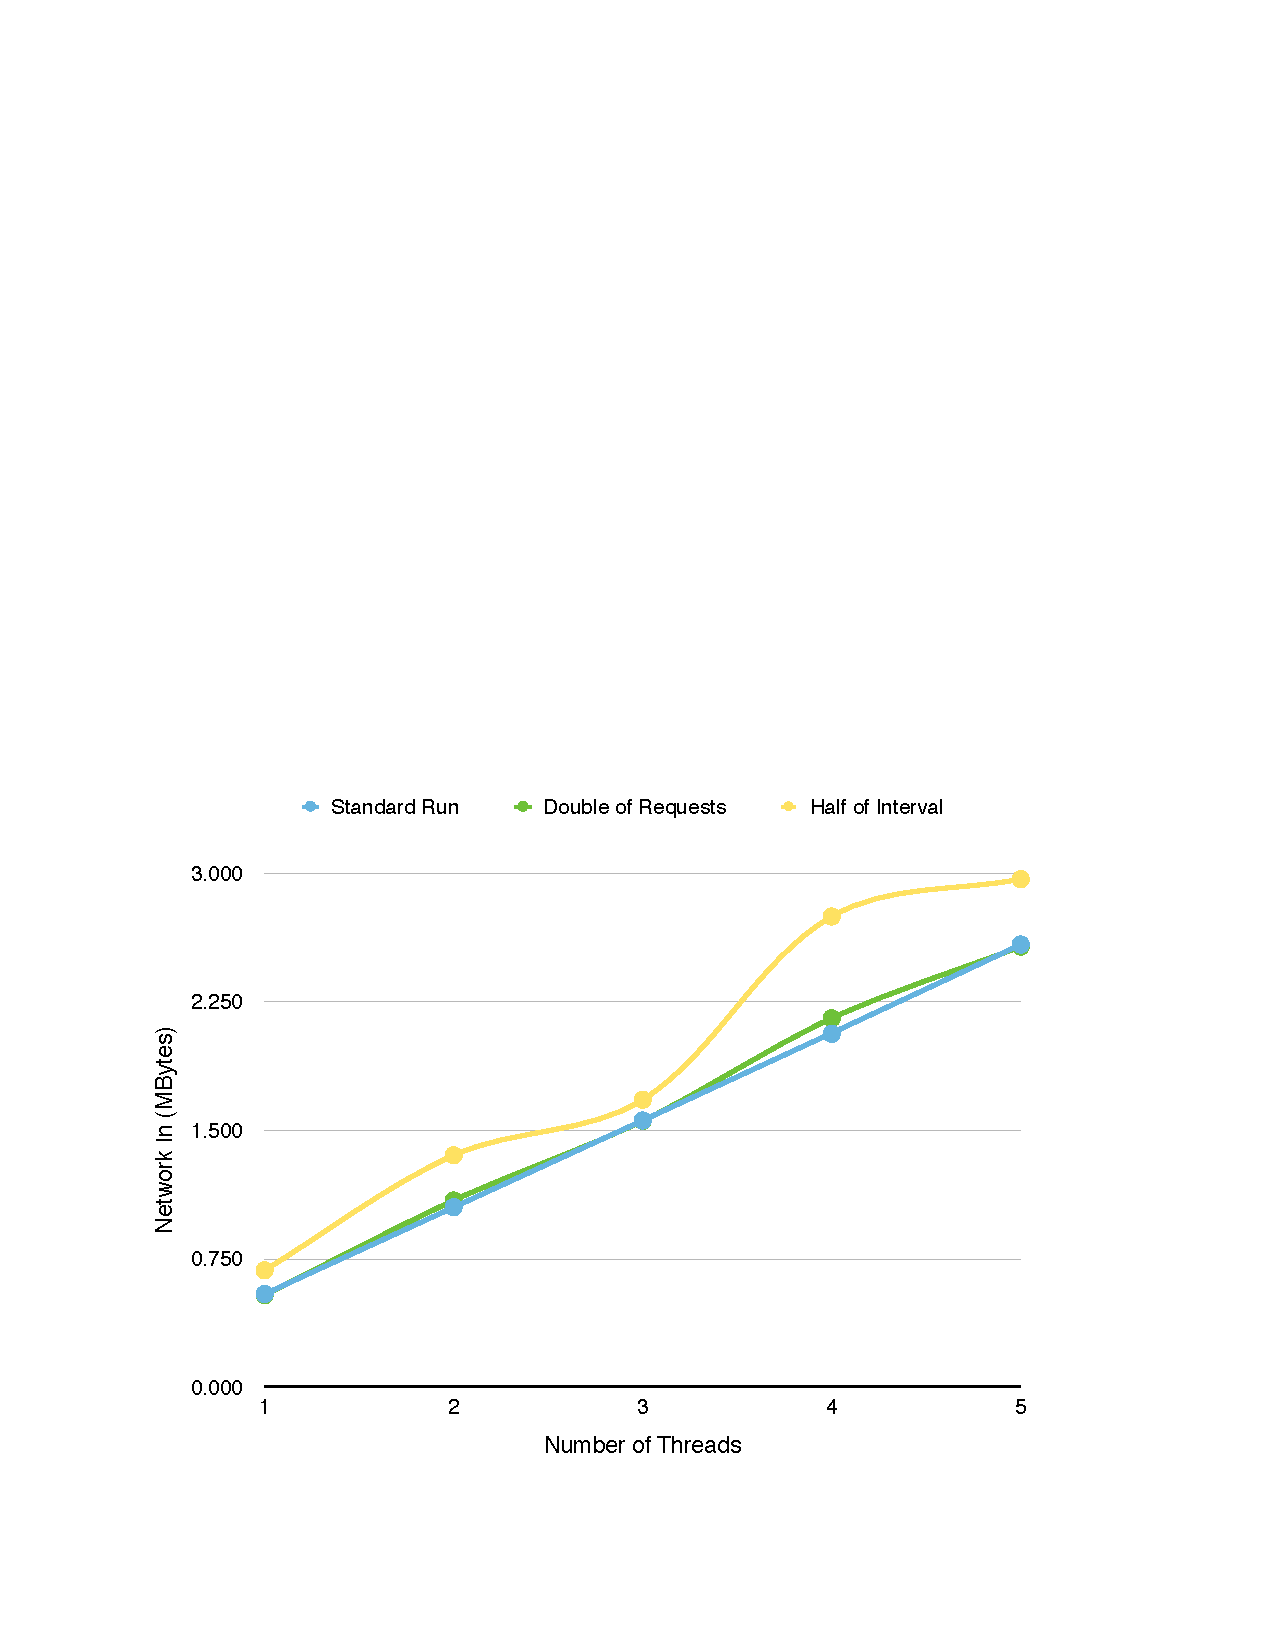
\includegraphics[width=\linewidth]{./images/network_1_lap}
  \caption{Baseline Network traffic.}
  \label{fig:eval_baseline_network}
\end{subfigure}
\caption{Baseline performance results.}
\label{fig:eval_baseline_results}
\end{figure}

Figure~\ref{fig:eval_baseline_cpu} presents the system metric \textit{CPU Utilization} for the current
experiment. Comparing the values obtained in the experiment for the three variations, for the
\textit{Standard} and the \textit{Double of Requests} variations the behavior is very similar and tend
to take a linear pattern. For the \textit{Half of Interval} variation, it is possible to observe
that in this variation, the metric value is always higher - maximum close to 16$\%$ - compared with the other
variations. The metric behavior changes according the number of threads that are sending events and
tend to take a sinusoidal pattern.\\

The system metric \textit{Network In}, presented in Figure~\ref{fig:eval_baseline_network}, assumes a
similar behavior to the previous metric. For the \textit{Standard} and \textit{Double of Requests} variations,
the values are similar and the behavior tend to take a linear pattern. It is possible to take the same
conclusions for the \textit{Half of Interval} variation, where the values are always higher - maximum
close to 3 \gls{MB} - and the behavior tends to take a sinusoidal pattern.

\subparagraph{Track 3 Laps}
\label{subp:eval_exp_data_3laps}
In the \textbf{Track 3 Laps} scenario the session contains the data recorded based in the events generated
during 3 laps in the track. The parameters used to execute the test for this scenario are described in
Table~\ref{tab:3laps_parameters}.\\

% 3 Lap parameters
\begin{table}[ht!]
  \begin{tabular}{|c|c|}
    \hline
    Number of Events & Period \\ \hline
    8895             & 57ms   \\ \hline
  \end{tabular}
  \caption{3 Lap evaluation parameters.}
  \label{tab:3laps_parameters}
\end{table}

% 3 Lap results
\begin{figure}[ht!]
\centering
\begin{subfigure}{.5\textwidth}
  \centering
  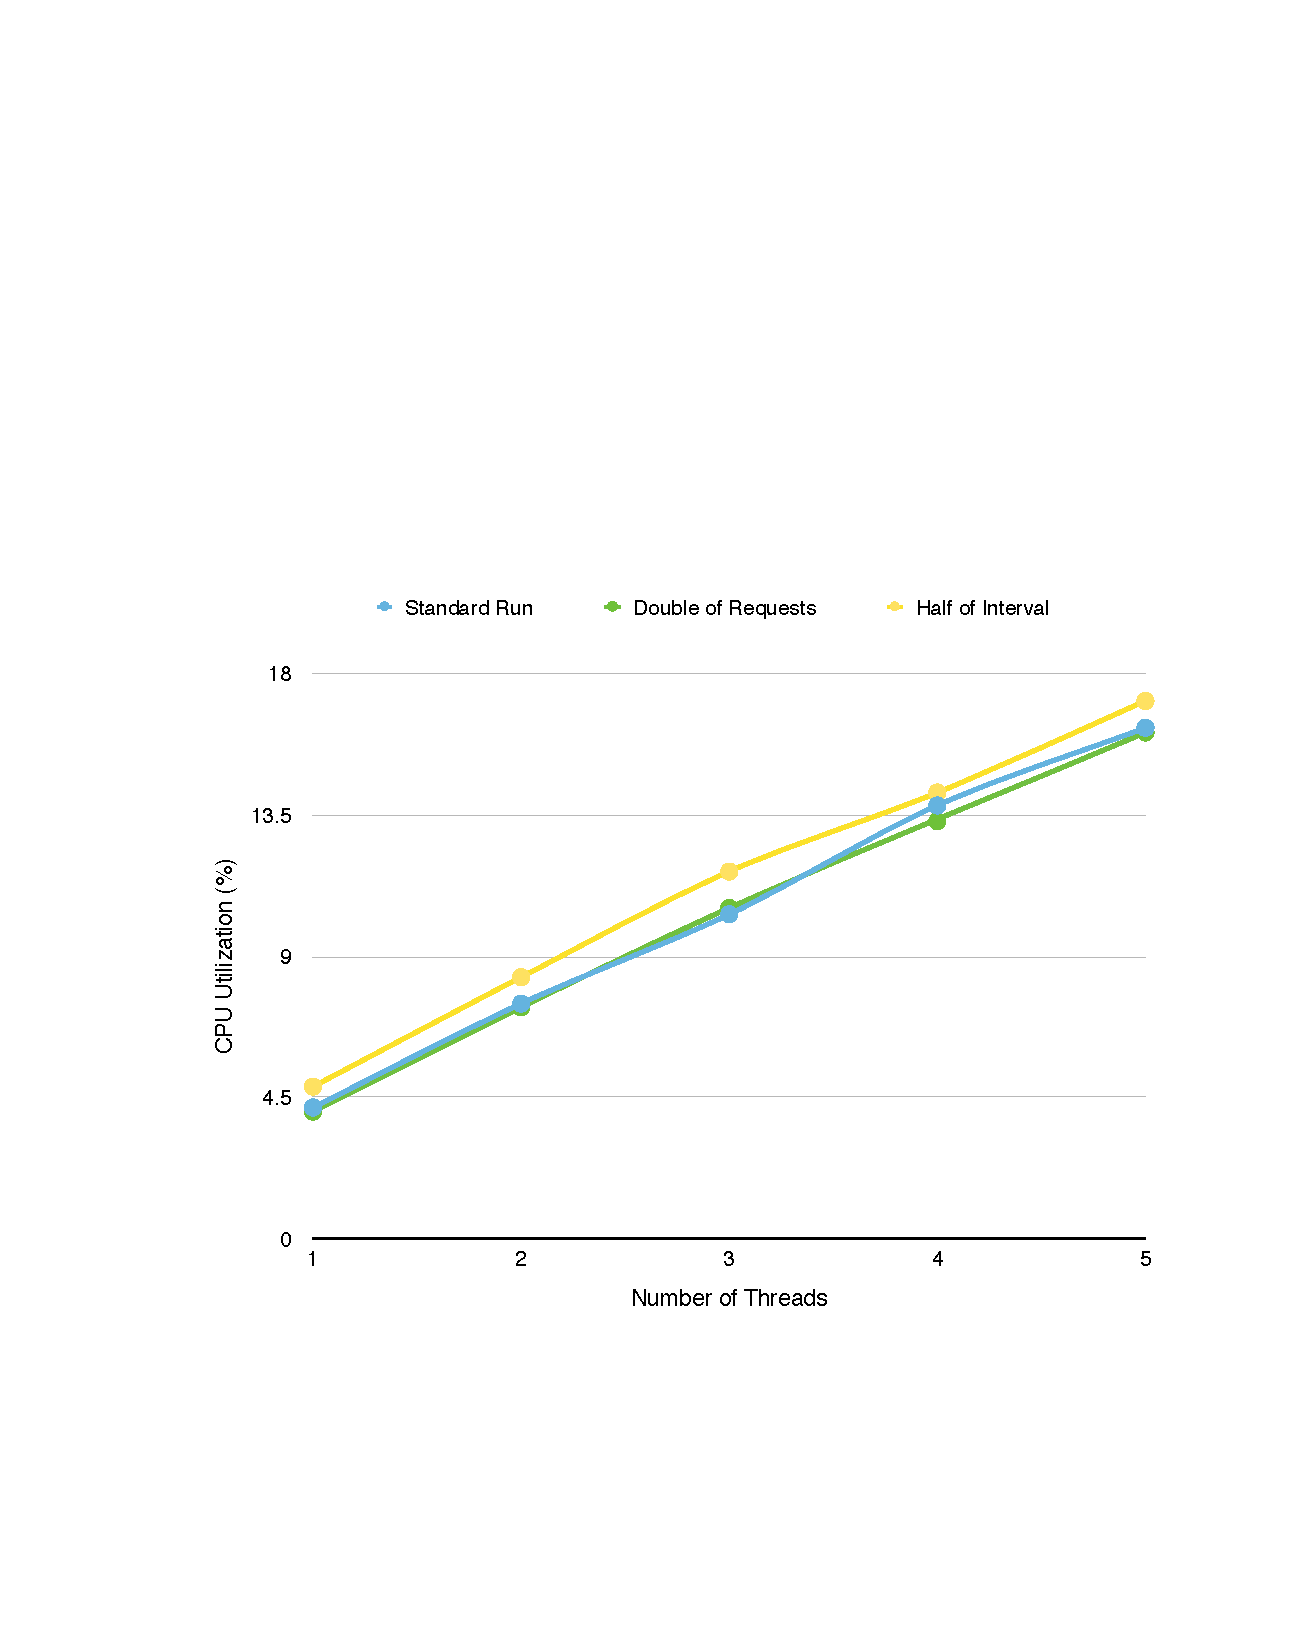
\includegraphics[width=\linewidth]{./images/cpu_3_lap}
  \caption{Track 3 Laps CPU Utilization.}
  \label{fig:eval_3laps_cpu}
\end{subfigure}%
\begin{subfigure}{.5\textwidth}
  \centering
  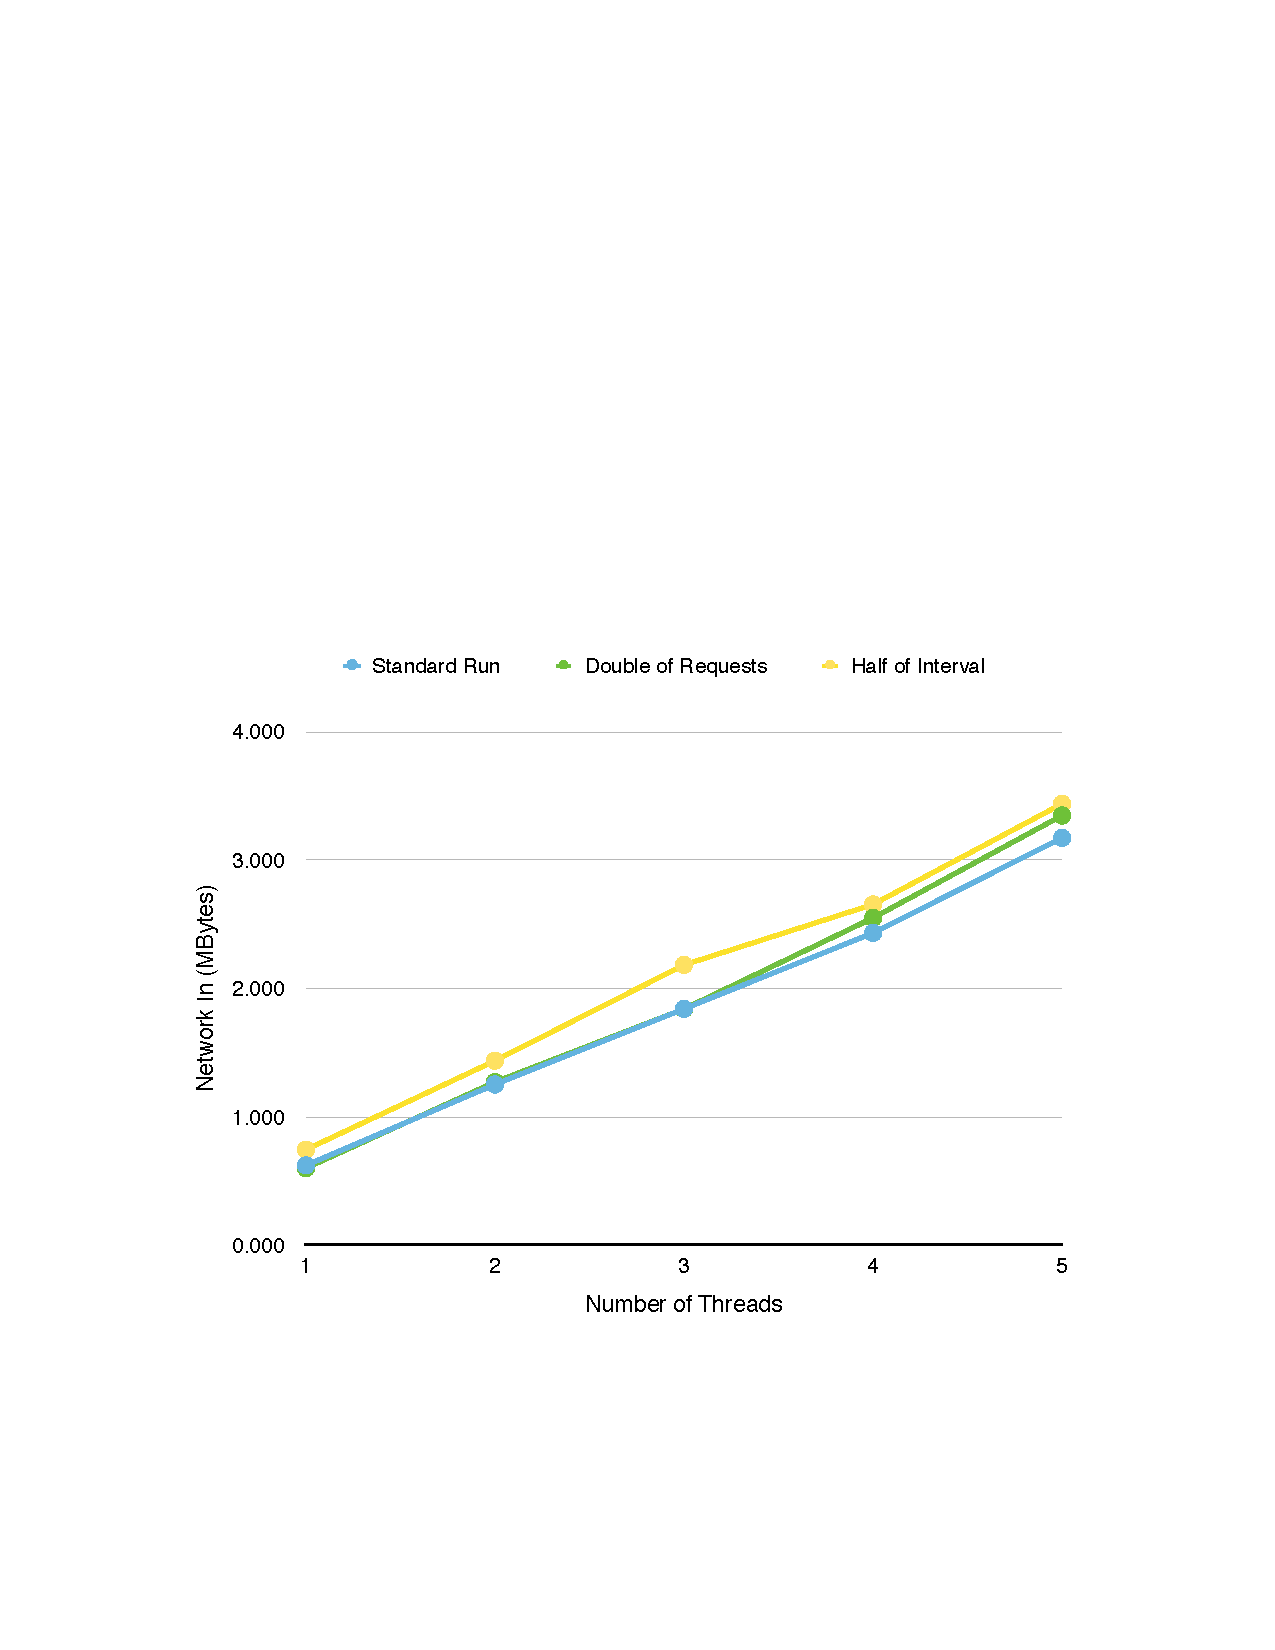
\includegraphics[width=\linewidth]{./images/network_3_lap}
  \caption{Track 3 Laps Network traffic.}
  \label{fig:eval_3laps_network}
\end{subfigure}
\caption{Track 3 Lap performance results.}
\label{fig:eval_3laps_results}
\end{figure}

Figure~\ref{fig:eval_3laps_cpu} presents the system metric \textit{CPU Utilization} for the current
experiment. Comparing the values values obtained in the experiment, it is possible to observe that
the values are very similar for all variations. The \textit{Half of Interval} continues to present
the highest values - maximum close to 18$\%$ - while the other variations presents almost identical
values. Regarding the metric behavior, all variations tends to take a linear pattern.\\

As in the previous experiment, the system metric \textit{Network In}, presented in Figure~\ref{fig:eval_3laps_network},
is very similar to the previous regarding its values and behavior. The \textit{Half of Interval}
variation still presents the highest values - maximum close to 3.5 \gls{MB} - but as the number of
threads increase, it is possible to observe that the values of the \textit{Double of Requests}
variation tend to be close to the \textit{Half of Interval} variation.


\subsection{Latency Interaction}
\label{sub:eval_exp_latency}
To evaluate the latency interaction for an event that occurs in the smart place and the corresponding
action that is triggered in the smart place, we use the scenario where a tagged robot was programmed to
execute a given number of laps in the warehouse plant where \gls{RFID} readers are placed to detect
when the robot is approaching. During the lap the robot stops during 5 seconds near to a reader and
then continues its lap.\\

According the methodology described in Section~\ref{sub:eval_methodology_latency}, the smart place
network connection was monitored to allow the inspection of incoming and outgoing connections and
determine how the connection time is spent in the cloud-based approach and the fog-based approach,
based on the proposed metrics. In our simulation the smart place was monitored through the
\textit{tcpdump}\footnote{http://www.tcpdump.org/} tool, that allows to monitoring the packets that
are being transmitted or received over a network.\\

The simulation was performed according two different specifications for the \gls{ALE} module,
\textit{Base Event Cycle} and \textit{Half-period Event Cycle} .

% Standard Event Cycle
\subparagraph{Baseline Event Cycle}
\label{subp:eval_exp_latency_ecspec}
 In the baseline scenario, we define the \textit{Base ECspec} to configure the \gls{ALE} module. The
 configuration parameters are described in Table~\ref{table:ecspec_base}.

% Base ECspec parameters
 \begin{table}[ht!]
   \begin{tabular}{|c|c|}
     \hline
     Period & Duration \\ \hline
     10s    & 9.5s     \\ \hline
  \end{tabular}
  \caption{Base ECspec parameters.}
  \label{table:ecspec_base}
 \end{table}

\begin{figure}[ht!]
  % ECSpec local breakdown figure
  \centering
  \begin{subfigure}{.5\textwidth}
    \centering
    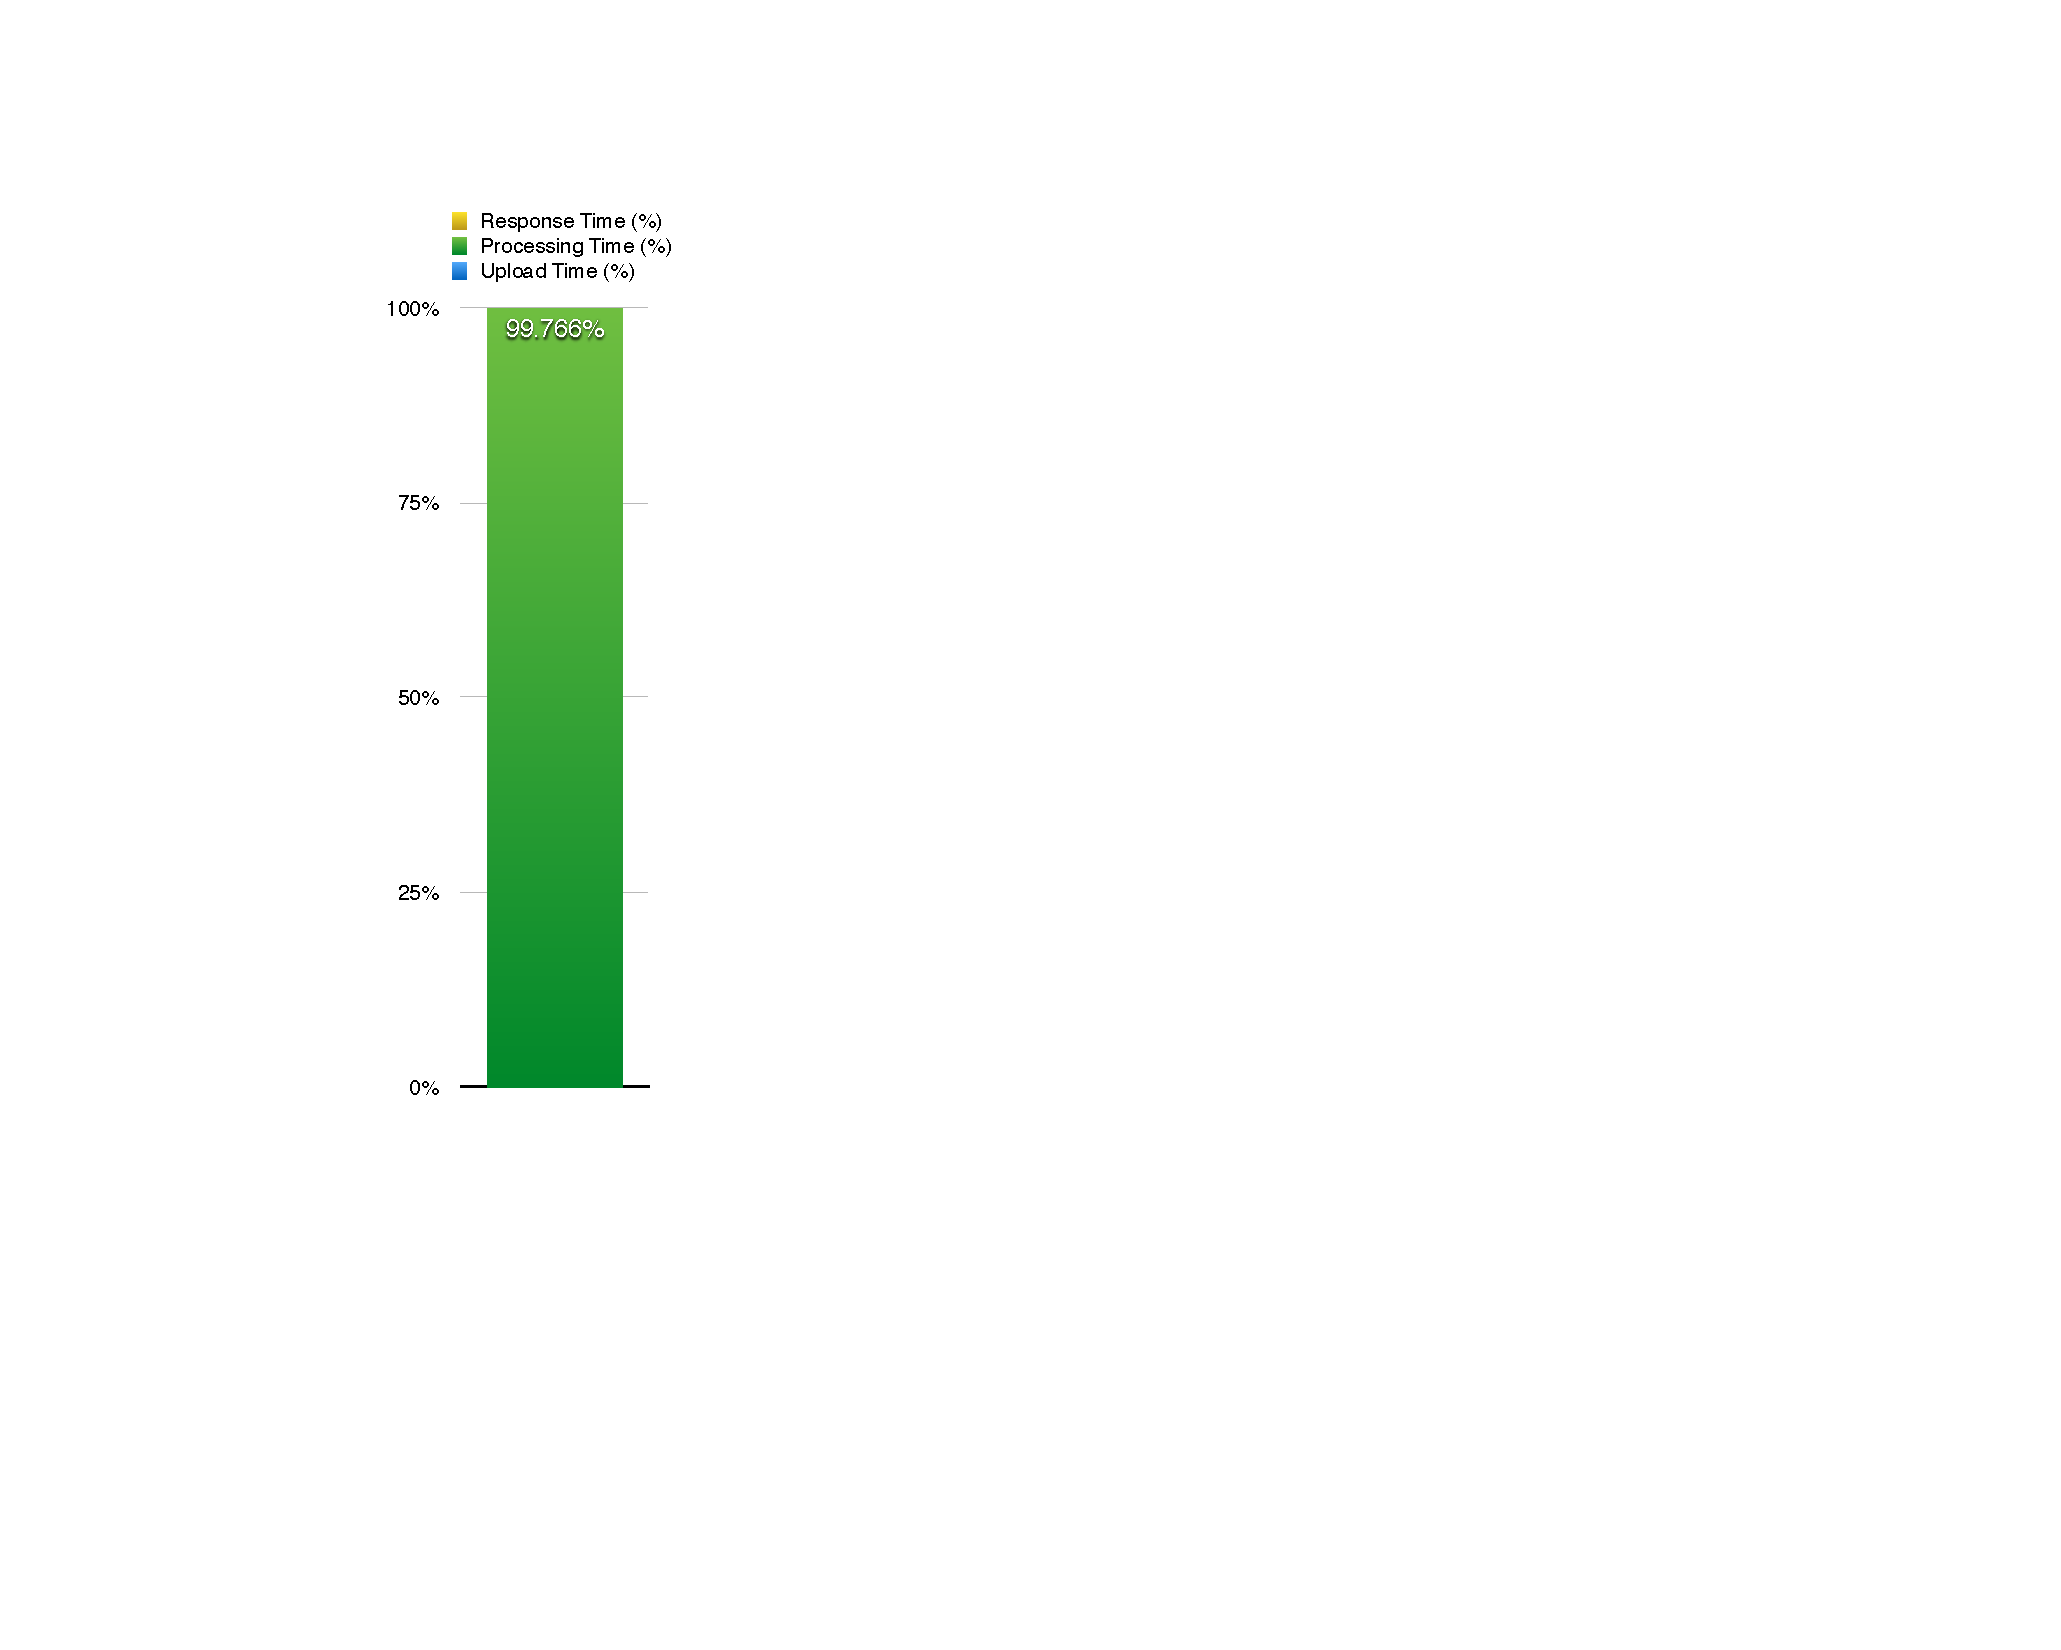
\includegraphics[width=.365\linewidth]{./images/ecspec_local_breakdown}
    \caption{Fog-based approach: baseline\\Event Cycle latency breakdown.}
    \label{fig:ecspec_local}
  \end{subfigure}%
  % ECSpec cloud breakdown figure
  \begin{subfigure}{.5\textwidth}
    \centering
    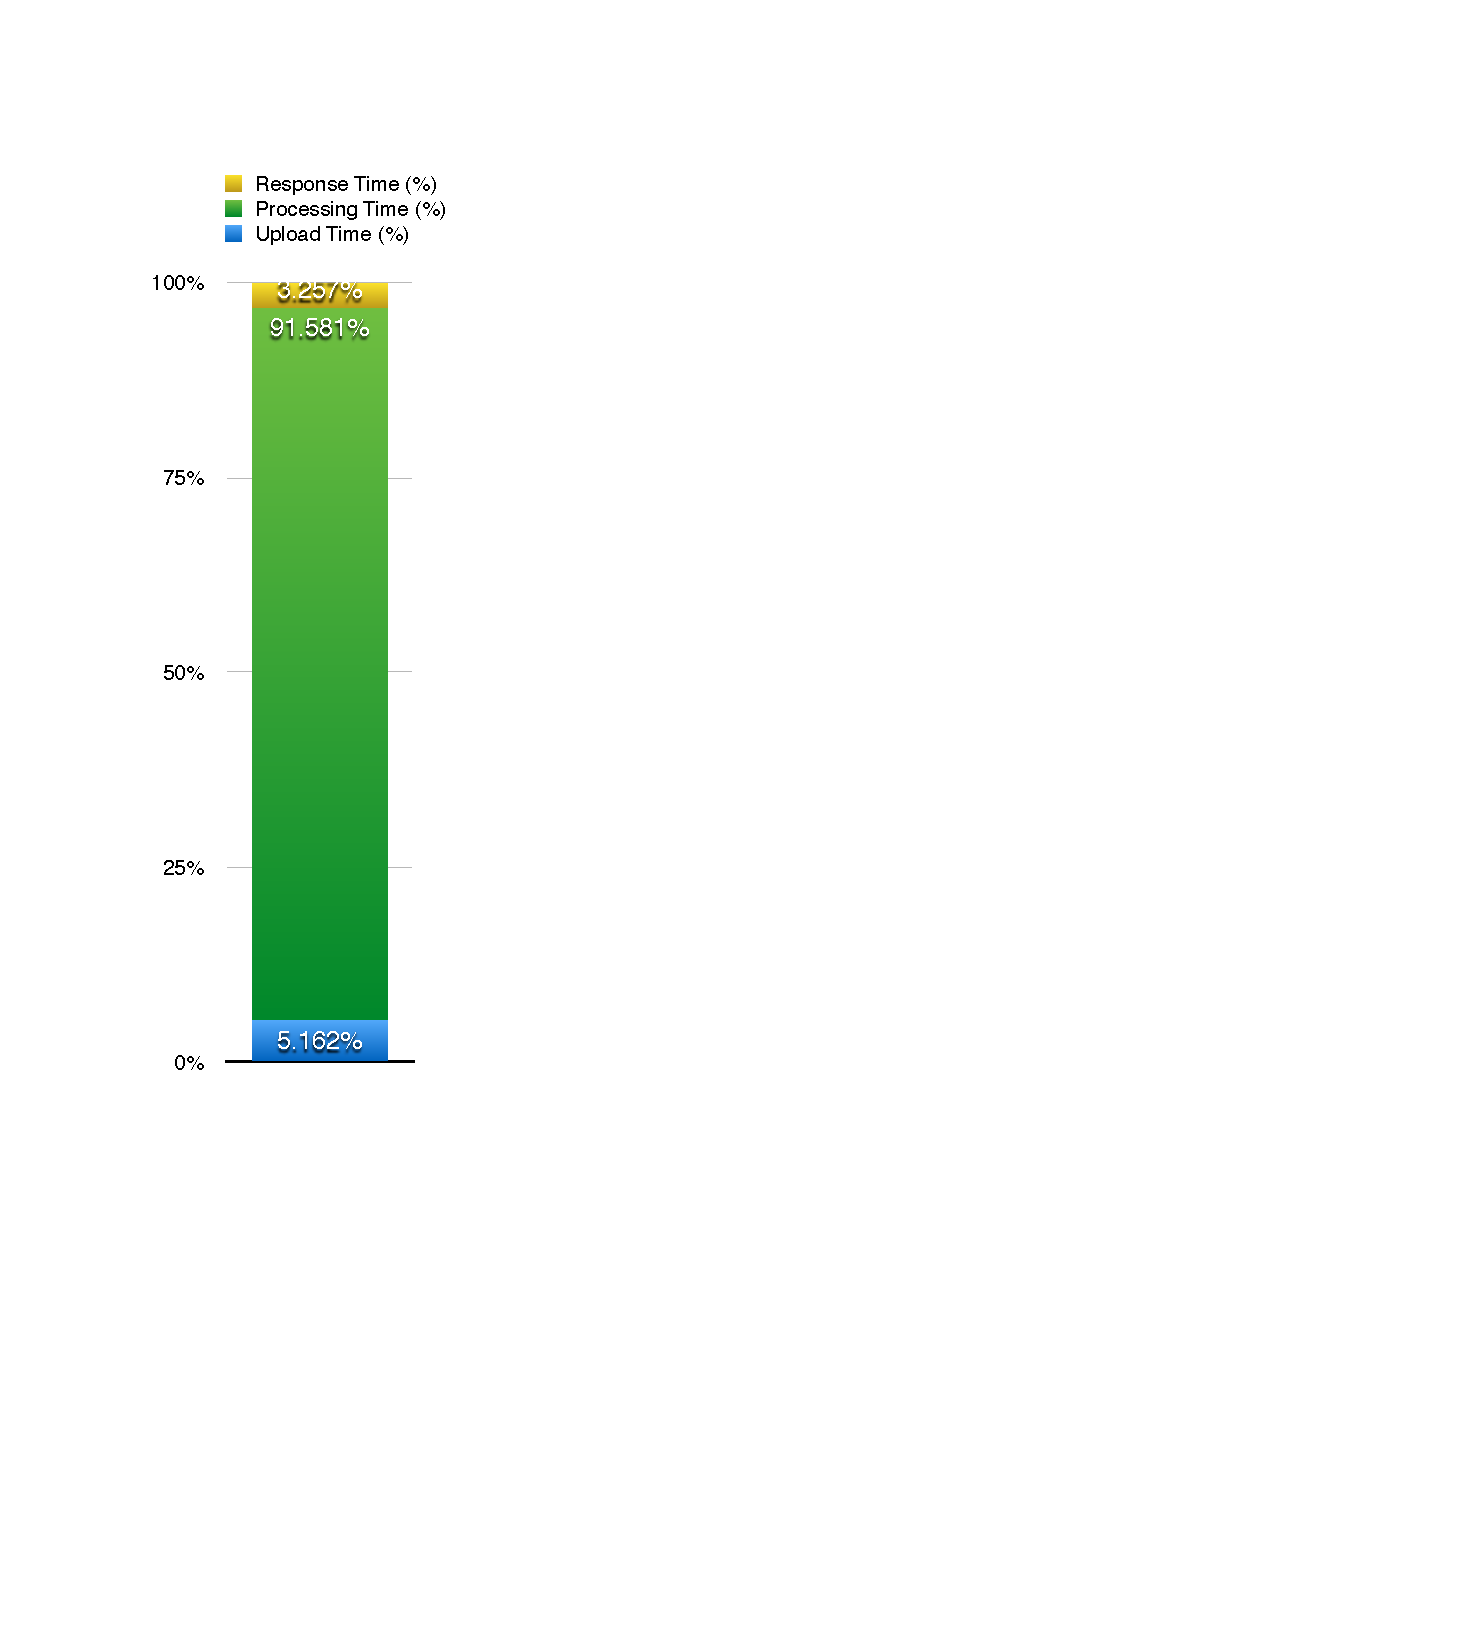
\includegraphics[width=.4\linewidth]{./images/ecspec_cloud_breakdown}
    \caption{Cloud-based approach: baseline\\Event Cycle latency breakdown.}
    \label{fig:ecspec_cloud}
  \end{subfigure}
  \caption{Baseline Event Cycle latency breakdown.}
  \label{fig:ecspec_breakdown}
\end{figure}

Figure~\ref{fig:ecspec_breakdown} presents the event latency breakdown for the current experiment.
Comparing the latency breakdown for the fog-based approach, presented in Figure~\ref{fig:ecspec_local},
with the cloud-based approach, presented in Figure~\ref{fig:ecspec_cloud}, it is possible to observe
that the value of the \textit{Upload Latency} and \textit{Response Latency} metrics for the cloud-approach
- close to 9$\%$ of the \textit{Event Latency} - is considerable higher when compared with the fog-approach,
where those values represent less then 0.5$\%$ of the \textit{Event Latency} metric. Is important to
point that the behavior for the \textit{Upload Latency} and \textit{Response Latency} metrics are
different for both approaches, in the fog-based approach the value of the \textit{Upload Latency}
metric is almost 50$\%$ higher then the \textit{Response Latency} metric, while in the cloud-based
approach those metrics presents the opposite behavior.\\

% % ECSpec local breakdown table
\begin{table}[ht!]
  \begin{tabular}{|c|c|c|c|c|}
  \hline
  ~                & Upload Time & Processing Time & Response Time & Event Latency \\ \hline
  Average Time (s) & 0.006       & 7.525           & 0.011         & 7.542         \\ \hline
  \end{tabular}
  \caption{Fog-based approach: baseline Event Cycle latency time.}
  \label{table:ecspec_local}
\end{table}

% % ECSpec cloud breakdown table
\begin{table}[ht!]
  \begin{tabular}{|c|c|c|c|c|}
  \hline
  ~                & Upload Time & Processing Time & Response Time & Event Latency \\ \hline
  Average Time (s) & 0.310       & 7.763           & 0.228         &  8.301        \\ \hline
  \end{tabular}
  \caption{Cloud-based approach: baseline Event Cycle latency time.}
  \label{table:ecspec_cloud}
\end{table}

Table~\ref{table:ecspec_local} and Table~\ref{table:ecspec_cloud} presents the latency values for the
current experiment. The metric values for the fog-based approach were obtained through the average
of 11 events that were generated during the experiment, while the values for the cloud-based were
obtained through the average of 9 events. Comparing the latency values for both approaches,
immediately is possible to observe that there is a huge difference between the values of the
\textit{Upload Latency} and \textit{Response Latency} metrics between both approaches. That
difference reflects in the value of the \textit{Event Latency} metric, where the fog-based approach
is almost 1s faster then the cloud-based approach.

\subparagraph{Half-Period Event Cycle}
\label{subp:eval_exp_latency_ecspec_fast}
In this scenario, we define the \textit{Half-period ECspec} to configure the \gls{ALE} module.
The configuration parameters are described in Table~\ref{table:ecspec_fast}.

% Half-period ECspec parameters
\begin{table}[ht!]
  \begin{tabular}{|c|c|}
    \hline
    Period & Duration \\ \hline
    5s    & 4.75s     \\ \hline
  \end{tabular}
  \caption{Half-period ECspec parameters.}
  \label{table:ecspec_fast}
\end{table}

\begin{figure}[ht!]
  \centering
  % ECSpec Fast local breakdown figure
  \begin{subfigure}{.5\textwidth}
    \centering
    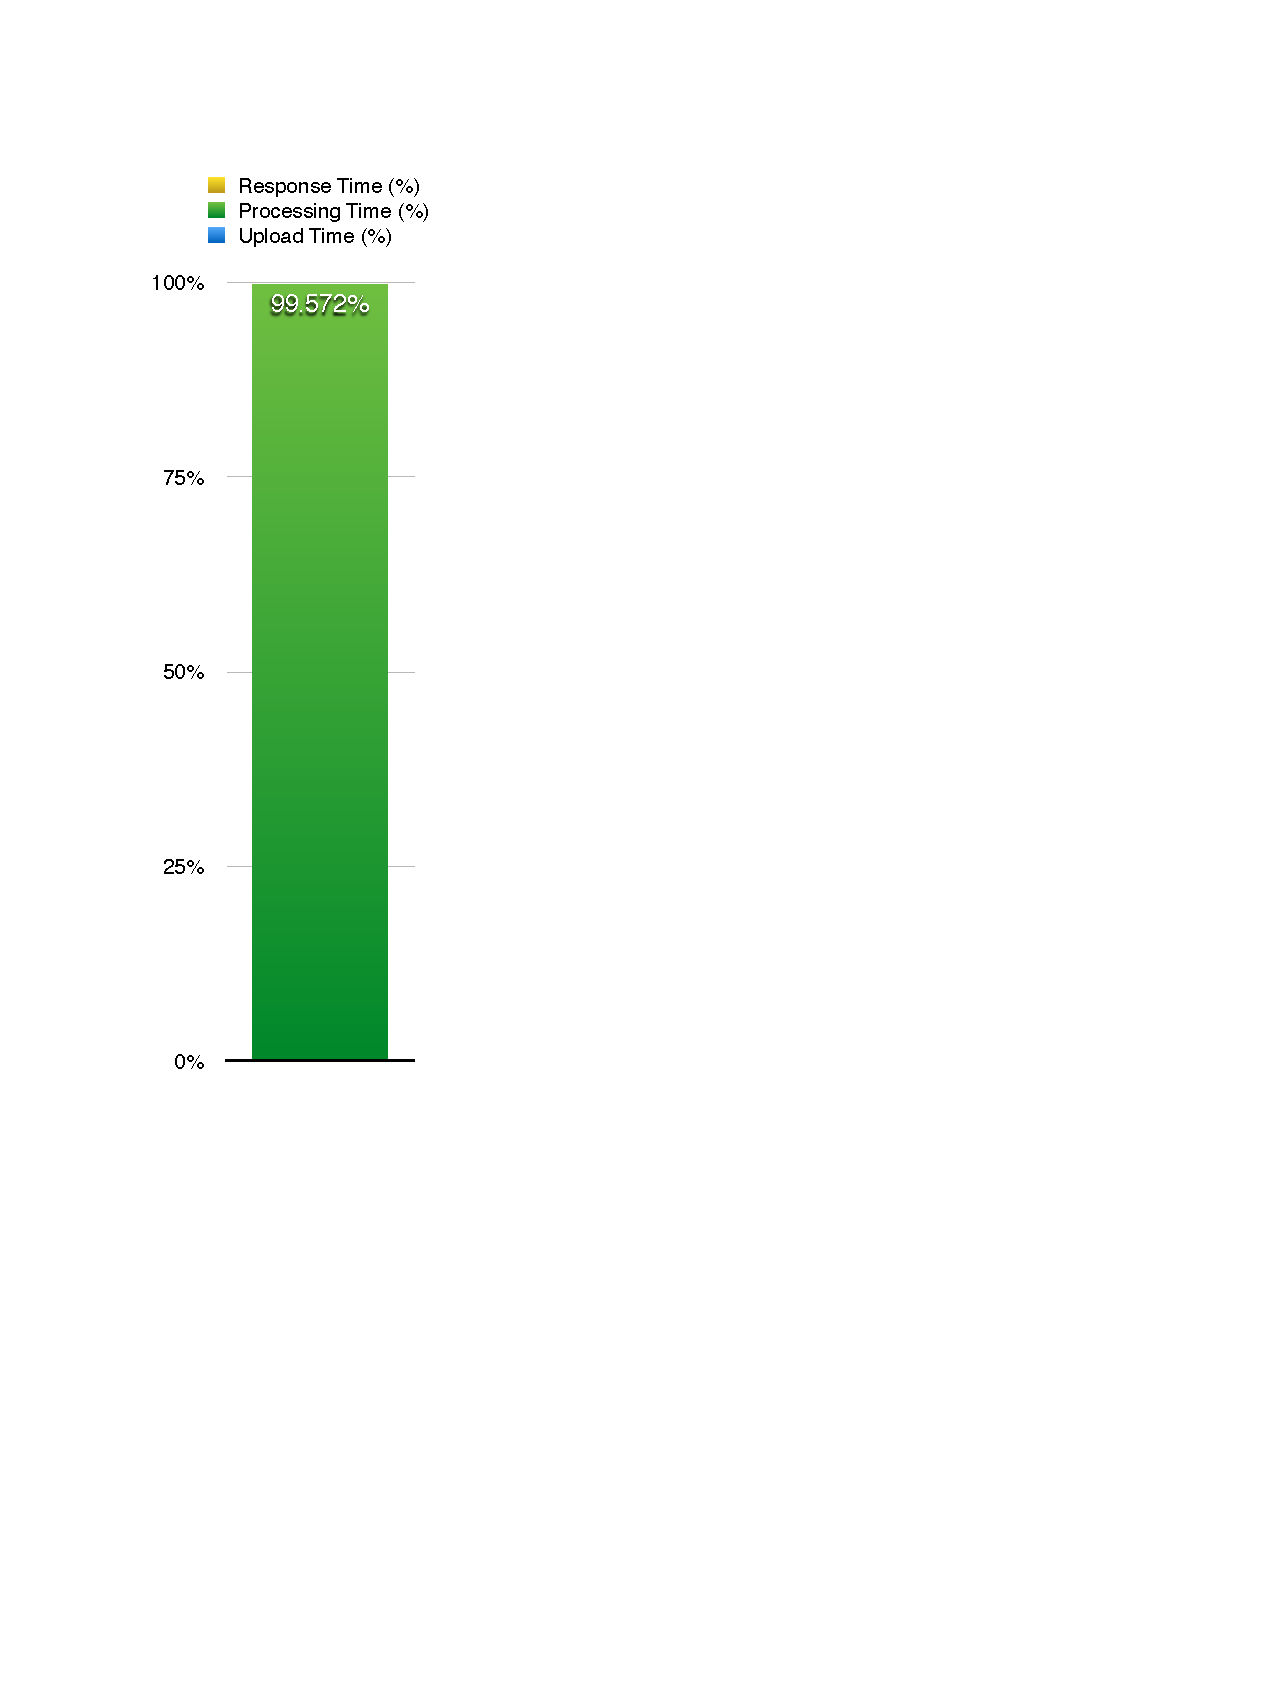
\includegraphics[width=.4\linewidth]{./images/ecspec_fast_local_breakdown}
    \caption{Fog-based approach: half-period Event Cycle\\ latency breakdown.}
    \label{fig:ecspec_fast_local}
  \end{subfigure}%
  % ECSpec fast cloud breakdown figure
  \begin{subfigure}{.5\textwidth}
    \centering
    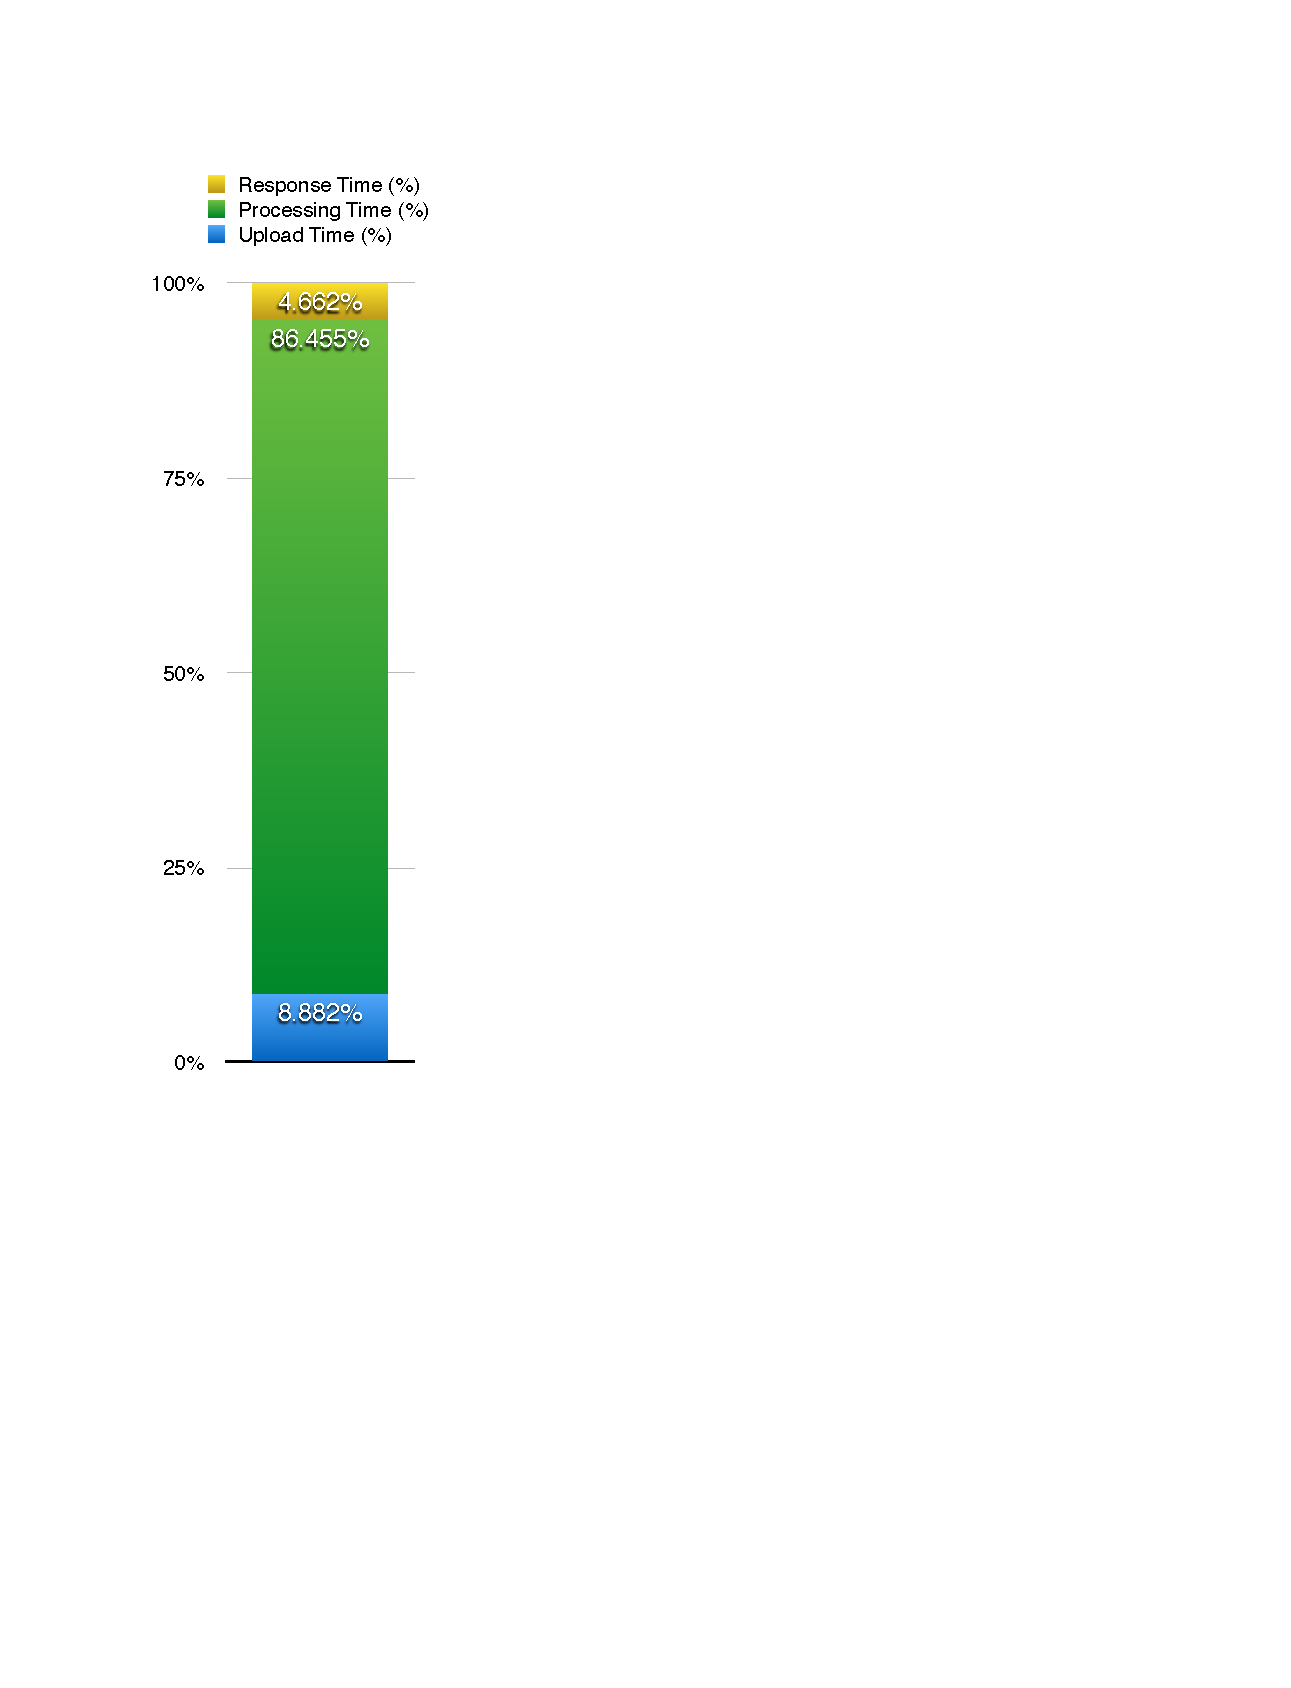
\includegraphics[width=.4\linewidth]{./images/ecspec_fast_cloud_breakdown}
    \caption{Cloud-based approach: half-period Event Cycle\\ latency breakdown.}
    \label{fig:ecspec_fast_cloud}
  \end{subfigure}
  \caption{Half-period Event Cycle latency breakdown.}
  \label{fig:ecspec_fast_breakdown}
\end{figure}

Figure~\ref{fig:ecspec_fast_breakdown} presents the event latency breakdown for the current experiment.
Comparing the latency breakdown for the fog-based approach, presented in Figure~\ref{fig:ecspec_fast_local},
with the cloud-based approach, presented in Figure~\ref{fig:ecspec_fast_cloud}, as in the previous experiment
it is possible to observe that the values of the \textit{Upload Latency} and \textit{Response Latency}
metrics for the cloud-approach are higher - close to 14$\%$ of the \textit{Event Latency} metric - to
the obtained in the \textit{Baseline} experiment, while the values obtained for the fog-approach
- close to 0.5$\%$ - maintained similar values. Regarding the behavior for those metrics, compared
with the \textit{Baseline} experiment, the behavior pattern observed in the previous experiment
was maintained.

% % ECSpec fast local breakdown table
\begin{table}[ht!]
  \begin{tabular}{|c|c|c|c|c|}
  \hline
  ~                & Upload Time & Processing Time & Response Time & Event Latency \\ \hline
  Average Time (s) & 0.006       & 4.216           & 0.010         & 4.232         \\ \hline
  \end{tabular}
  \caption{Fog-based approach: half-period Event Cycle latency time.}
  \label{table:ecspec_fast_local}
\end{table}

% % ECSpec fast cloud breakdown table
\begin{table}[ht!]
  \begin{tabular}{|c|c|c|c|c|}
  \hline
  ~                & Upload Time & Processing Time & Response Time & Event Latency \\ \hline
  Average Time (s) & 0.313       & 3.578           &  0.177        & 4.068         \\ \hline
  \end{tabular}
  \caption{Cloud-based approach: half-period Event Cycle latency time.}
  \label{table:ecspec_fast_cloud}
\end{table}

Table~\ref{table:ecspec_fast_local} and Table~\ref{table:ecspec_fast_cloud} present the latency values for the
current experiment. The metric values for the fog-based approach were obtained through the average
of 20 events that were generated during the experiment, while the values for the cloud-based were
obtained through the average of 23 events. As in the \textit{Baseline} experiment, the latency values
of the \textit{Upload Latency} and \textit{Response Latency} metrics presents a significant difference
between both approaches, where the values for the cloud-based approach continues to be higher.
However, in this experiment the fog-based approach present higher values for the \textit{Event Latency}
metric. Comparing the values presented in Table~\ref{table:ecspec_fast_local} and Table~\ref{table:ecspec_fast_cloud},
is possible to observe that the cause for that was the result tof he \textit{Processing Time}
metric, where the fog-based approach presented a better than the cloud-based approach.

% Evaluation Analysis
\section{Results Analysis and Discussion}
\label{sec:eval_analysis}
Based on the results obtained and in the requirements of application domains, it is possible to specify
which is the most adequate approach to deploy a smart place application that relies on \gls{RFID}
technology and in the Fosstrak middleware.

% Data scalability
\subparagraph{Data Scalability.}
\label{subp:eval_results_data}
Regarding the data scalability for the Fosstrak middleware, is possible to conclude that the metrics
of \textit{CPU Utilization} and \textit{Network In} increase as the threads and requests are growing.
These results are concise with the ones obtained by Gomes et al. \cite{gomes2014future}, which
proposes a new \gls{IoT} infrastructure for \gls{EPC}Global middleware. Moreover, in the experiments
performed Gomes detected that when the \textit{CPU Utilization} crosses the value of 95$\%$, the
outbound traffic started to decrease. After an analyzing the stored data, they conclude that the
\gls{CPU} exhaustion caused by the \gls{EPCIS} affected the performance of \gls{ALE} module,
resulting in a delay of data storage in the \gls{EPCIS} repository, which explains the observed
behavior.

% Latency Interaction
\subparagraph{Latency Interaction.}
\label{subp:eval_results_latency}
Regarding the latency interaction, it is clear that the fog-approach presented a better performance
than the cloud-based approach. However, there is a clear trade-off when choosing one of the proposed
approaches. In one side, the fog-based approach guarantees a better overall performance for the smart
place when compared with the cloud-based approach.\\

However, it is important to point that there some aspects that can improve the overall performance
of the cloud-based approach. For instance, the network connection is a possible bottleneck for the
performance of such approach. We believe that if the experiments were conducted through a faster
network connection - e.g. a Fiber-optic connection - the overall performance of the cloud-approach
will be better, but not as the fog-based approach.\\

In the other side, the fog-based approach requires an infrastructure burden that a cloud-based approach
is able to suppress. This is an important aspect to take in consideration when choosing one of the
approaches, since that a fog-based approach requires a large investment in infrastructure and the
performance gain offered by such approach could not be so substantial when compared with a cloud-based
approach.\\

\subparagraph{Fog or Cloud?}
\label{subp:eval_conclusion}
The obtained results shows that a fog-based approach offers better performance to deploy a smart
warehouse application based in \gls{RFID} technology that requires low latency interaction.
But it will be this approach the best choice for all application domains?\\

Table \ref{table:smart_places_requirements} presents the requirements of \gls{IoT} applications
for several domains. For instance, for application domains with a small network size, low network
bandwidth requirements, low scalability and does not require low latency interaction - such as Smart
Home/Office and Smart Retail scenarios - a cloud-based approach is suitable, but probably the more adequate
solution it will be to provisioning the infrastructure in local, since that in most cases a local
server is able to host such applications.\\

For domains with a medium/large network size and network bandwidth requirements, that does not require
a low latency interaction but presents high scalability - such as Smart Agriculture and Smart Water
scenarios - a cloud-based approach is the most reasonable choice. Finally, for domains with a
medium/large network size and network bandwidth requirements, that requires low latency interaction
and presents high scalability - such as Smart Cities and Smart Transportation scenarios - the
fog-based approach is the best solution.


%!TEX root = ../dissertation.tex

% Conclusion
\section{Conclusion and Future Work}
\label{sec:conclusion}
The present work explored the deployment of \gls{IoT} applications for smart warehouses based on the
\gls{RFID} technology with two different approaches to deploy: one based in a traditional cloud
deployment approach (cloud-based) and other according the Fog Computing platform (fog-based). More
specifically, the present work focuses to determine if a cloud-based approach is able to meet the
low-latency requirements of many \gls{IoT} applications, since that low-latency is an essential
requirement of \gls{IoT} applications. If a cloud-based approach is not able to meet the network latency
requirements for those applications, the cloud platform is not a viable option to perform the
provisioning of \gls{IoT} applications.

To improve the provisioning of \gls{RFID} middleware in the cloud, we developed a mechanism based on
Docker containers and the Chef tool that automates the installation and configuration of the modules
that composes the Fosstrak platform \gls{RFID} middleware. This mechanism was of extreme
importance, because it allowed us to perform the application provisioning of the cloud instances in
a very efficient way. Although our experiments were conducted in a single cloud provider, the developed
mechanism gave us the flexibility to choose between several cloud providers to provision the
\gls{RFID} middleware.

Regarding the system evaluation, we defined two methodologies for evaluate the latency of an event that
occurs in the physical space and the data storage performance for the Fosstrak platform. With the
methodologies proposed, we were able to compare the event latency performance for both cloud-based
and fog-based approaches. We defined two experiments to evaluate the latency performance of the
deployment approaches. The obtained results shows that the event latency performance presented better
results when the application was deployed according the fog-based approach. However, we identified
some issues regarding the behavior of a Fosstrak module (\gls{ALE}) that affected the performance
of the event latency for both deployment approaches. Regarding the data storage performance of the
RFID middleware, the results show that the Fosstrak platform is able to process with an acceptable
performance the amount of data that is generated in a smart warehouse.

% Future Work
\subsection{Future Work}
\label{sub:future_work}
In the present work, we achieved our initial goals and determine that a fog-based approach is more
adequate to deploy a smart place application based in \gls{RFID} technology. However, our solution
is not perfect and there some aspects that can be improved in the future.

Our solution proposes that the \gls{RFID} application is deployed following a fog-based approach.
This means that we need to have a cloud close to the ground and this cloud must meet the same
requirements of a remote cloud such as high scalability, security and multi-tenancy. Unfortunately,
we were not able to implement a fog that meet these requirements and in our implementation the fog
was built on top of a traditional Virtual Machine. In the future, the fog needs to be correctly
implemented providing all the features of the remote cloud and in addition features such as
location-awareness, mobility support and geo-distribution.

In the current implementation we used Docker containers to provisioning the Fosstrak software stack.
In the evaluation of our solution we deploy the containers in a \gls{EC2} \gls{VM}, which overlays two
different mechanisms of virtualization. Although we still are able to take advantage of some benefits
from the containers such as the portability, other benefits such as the low I/O and disk space are
hidden by the \gls{VM} hypervisor. A future improvement that can be made is to perform the deployment
of the containers on top of the bare-metal or in a cloud-based container service - e.g. Google Kubernetes
\footnote{\url{http://kubernetes.io/}} or \gls{AWS} \gls{EC2} Container Service\footnote{\url{https://aws.amazon.com/ecs/}} -
in order to improve the overall performance of the solution.

Regarding the system evaluation, it was performed only in \gls{AWS} \gls{EC2} instances. For the future
is important to evaluate our solution in other cloud providers to compare which offers the best cost/performance
relation. Also, in experiments performed to evaluate the latency interaction, we defined only two
different \textit{ECspecs}. For the future work, we want to evaluate the latency performance for
our solution with \textit{ECspecs} that presents smaller periods in order to determine which
specification is more suitable for our solution.

In the evaluation scenario we used a virtual RFID reader instead of a physical one, which
does not allow reproducing the environment conditions of a real smart warehouse such as interferences
in the RFID tags antennas, network bandwidth variations, etc. However, in the evaluation experiments
we used for some experiments traces from the work developed by Correia et. al \cite{Correia:Thesis:2014},
which have the real data traces mentioned above. A future improvement is to conduct the system evaluation
in a real scenario in order to have more accurate results.

Finally, the Utility Computing allows to leverage the smart place infrastructure to the cloud,
where the resources are available in a pay-as-you-use model. However, there is a
trade-off between performance and costs. By leveraging the smart place infrastructure
to the cloud, we can reduce the costs of the smart place operation, but the
application performance can be compromised. For the future work, we want to perform
an analysis to establish the relation between the performance and cost of a smart place
regarding its deployment approach: cloud, fog and local. This analysis will allow
to choose which is the most adequate approach to deploy an smart place based in
the performance of the application and the costs of the smart place operation.


\NewPage

\bibliographystyle{ieeetr}
\addcontentsline{toc}{chapter}{Bibliography}
\bibliography{bibliography/dissertation}

% Appendix
\appendix
%!TEX root = ../dissertation.tex

\chapter{Smart Place Requirements}
\label{appendix:smart_place_requirements}

% Smart Places requirements table
\begin{landscape}
  \begin{table}[p]
    \centering
    \begin{adjustbox}{width=\textwidth}
      \begin{tabular}{*{14}{l}}
      \toprule
      ~                      & \multicolumn{2}{l}{Smart Home/Office}                                  & \multicolumn{2}{l}{Smart Retail}                                       & \multicolumn{2}{l}{Smart City}                                                      & \multicolumn{2}{l}{Smart Agriculture/Forest}                                  & \multicolumn{2}{l}{Smart Water}                                                              & \multicolumn{2}{l}{Smart Transportation}                                             \\
      \midrule
      Network Size           & \multicolumn{2}{p{\colWidth}}{\raggedright Small}                      & \multicolumn{2}{p{\colWidth}}{\raggedright Small}                      & \multicolumn{2}{p{\colWidth}}{\raggedright Medium}                                  & \multicolumn{2}{p{\colWidth}}{\raggedright Medium/Large}                      & \multicolumn{2}{p{\colWidth}}{\raggedright Large}                                            & \multicolumn{2}{p{\colWidth}}{\raggedright Large}                                    \\
      Users                  & \multicolumn{2}{p{\colWidth}}{\raggedright Very Few, family members}   & \multicolumn{2}{p{\colWidth}}{\raggedright Few, community level}       & \multicolumn{2}{p{\colWidth}}{\raggedright Many, policy makers and general public}  & \multicolumn{2}{p{\colWidth}}{\raggedright Few, policy makers and landowners} & \multicolumn{2}{p{\colWidth}}{\raggedright Few, government}                                  & \multicolumn{2}{p{\colWidth}}{\raggedright Large, general public}                    \\
      Energy                 & \multicolumn{2}{p{\colWidth}}{\raggedright Rechargeable battery}       & \multicolumn{2}{p{\colWidth}}{\raggedright Rechargeable battery}       & \multicolumn{2}{p{\colWidth}}{\raggedright Rechargeable battery, Energy Harvesting} & \multicolumn{2}{p{\colWidth}}{\raggedright Energy Harvesting}                 & \multicolumn{2}{p{\colWidth}}{\raggedright Energy Harvesting}                                & \multicolumn{2}{p{\colWidth}}{\raggedright Rechargeable battery, Energy Harvesting}  \\
      Internet Connectivity  & \multicolumn{2}{p{\colWidth}}{\raggedright Wifi, 3G, 4G LTE, backbone} & \multicolumn{2}{p{\colWidth}}{\raggedright Wifi, 3G, 4G LTE, backbone} & \multicolumn{2}{p{\colWidth}}{\raggedright Wifi, 3G, 4G LTE, backbone}              & \multicolumn{2}{p{\colWidth}}{\raggedright Wifi, Satellite Communication}     & \multicolumn{2}{p{\colWidth}}{\raggedright Wifi, Satellite Communication, Microwave Links}   & \multicolumn{2}{p{\colWidth}}{\raggedright Wifi, Satellite Communication}            \\
      Data Management        & \multicolumn{2}{p{\colWidth}}{\raggedright Local Server}               & \multicolumn{2}{p{\colWidth}}{\raggedright Local Server}               & \multicolumn{2}{p{\colWidth}}{\raggedright Shared Server}                           & \multicolumn{2}{p{\colWidth}}{\raggedright Local Server, Shared Server}       & \multicolumn{2}{p{\colWidth}}{\raggedright Shared Server}                                    & \multicolumn{2}{p{\colWidth}}{\raggedright Shared Server}                            \\
      IoT Devices            & \multicolumn{2}{p{\colWidth}}{\raggedright RFID, WSN}                  & \multicolumn{2}{p{\colWidth}}{\raggedright Smart Retail}               & \multicolumn{2}{p{\colWidth}}{\raggedright RFID, WSN}                               & \multicolumn{2}{p{\colWidth}}{\raggedright WSN}                               & \multicolumn{2}{p{\colWidth}}{\raggedright Single Sensors}                                   & \multicolumn{2}{p{\colWidth}}{\raggedright RFID, WSN, Single Sensors}                \\
      Bandwidth Requirements & \multicolumn{2}{p{\colWidth}}{\raggedright Small}                      & \multicolumn{2}{p{\colWidth}}{\raggedright Small}                      & \multicolumn{2}{p{\colWidth}}{\raggedright Large}                                   & \multicolumn{2}{p{\colWidth}}{\raggedright Medium}                            & \multicolumn{2}{p{\colWidth}}{\raggedright Medium}                                           & \multicolumn{2}{p{\colWidth}}{\raggedright Medium/Large}                             \\
      \bottomrule
      \end{tabular}
    \end{adjustbox}
    \caption{Smart Place applications requirements.}
    \label{table:smart_places_requirements}
  \end{table}
\end{landscape}


% Glossary and Acronym List
\if\includeGlossary 1
\printglossary
\fi

\end{document}
